\documentclass{article}

\usepackage[margin=1.5cm, includefoot, footskip=30pt]{geometry}

%\usepackage{minted}  % would prefer to use minted but arxiv cannot shell-escape
\usepackage[T1]{fontenc}
\usepackage{amsmath}
\usepackage{booktabs}
\usepackage{graphicx}
\usepackage{hyperref}
\usepackage{listings}
\usepackage{lmodern}
\usepackage{multicol}
\usepackage{standalone}
\usepackage{xcolor}
\usepackage{subcaption}

\usepackage{tikz}
\usetikzlibrary{calc, shapes, patterns}

\title{Reviving, reproducing and revisiting Axelrod's second tournamentt}

\begin{document}

\maketitle

\section{Introduction}\label{sec:introduction}

The Prisoner's Dilemma has been the centre of the study of
cooperative behaviour since Robert Axelrod's seminal work in the
1980s~\cite{Axelrod1980a, Axelrod1980b, Axelrodbook}. In this work, Robert
Axelrod invited fellow academics to write computer code to play the Iterated
Prisoner's Dilemma. This initial research has subsequently led to a huge area
of research aiming to understand the emergence of cooperative behaviour. A good
overview of the variety of research areas is given in~\cite{Nowak2006}.

In the Prisoner's Dilemma, each player chooses
simultaneously and independently
between cooperation (C) or defection (D). The payoffs of
the game are defined by the matrix
\(
\begin{pmatrix}
    R & S \\ 
    T & P
\end{pmatrix}
\),
where $T > R > P > S$ and $2R > T + S$. The PD is a one
round game, but is commonly studied in a manner where the prior outcomes
matter. This repeated form is called the Iterated Prisoner's
Dilemma (IPD).


In Robert Axelrod's tournaments the particular values of \(R=3, P=1, S=0, T=5\)
were used.  Strategies were submitted written in either Fortran or Basic
% TODO Add a citation for bother languages
(in which case they were translated to Fortran). The very first
tournament~\cite{Axelrod1980a} involved 14 submissions  (complemented by a
fifteenth random strategy). Famously, the winner of this tournament was
Tit For Tat: a strategy that mimics the opponent's previous action. The only
sources for this work are the paper itself, all of the source code is apparently
lost. In the second tournament~\cite{Axelrod1980b} 64 strategies were submitted
and again: Tit For Tat was declared the winner. From a computation archaeological
point of view this tournament was far superior as the source code for all the strategies was
kept and made available for use. It can be found at
\url{http://www-personal.umich.edu/~axe/research/Software/CC/CC2/TourExec1.1.f.html}.

This work describes the process of reviving and using these strategies in a
modern software framework (\cite{AxelrodProject}): a Python library with over
200 strategies and a large number of analytical procedures which has been used
in ongoing research~\cite{Harper2017, Knight2017}.

Importantly, reviving the strategies is not done
through a manual exercise of reverse engineering the Fortran code which would be
prone to mistakes. This is done by calling the original functions ensuring the
\textbf{best possible reproduction and analysis of Robert Axelrod's original
work}. This will be described in more detail in Section~\ref{sec:reviving}.

Results and further analyses pertaining to reproducing the tournament will be
given in Section~\ref{sec:reproducing}. Finally, Section~\ref{sec:revisiting}
will extend the analysis to include contemporary research topics:

\begin{itemize}
    \item Experimenting with adding one of over 196 other strategies
        from~\cite{AxelrodProject} to see how the results change.
    \item Training strategies to perform at a high level using Genetic Algorithms.
    \item Investigating the overall performance of Zero determinant
        strategies~\cite{Press2012}.
    \item Running a tournament with all considered strategies (more than 250).
\end{itemize}

This work contributes to the game theoretic literature by providing the first
exercise in reproducing reported results that have been at the core of the study
of cooperation. Furthermore it also provides a contemporary lens which, amongst
other things concludes with one of the largest Iterated Prisoner's Dilemma
tournaments.
Finally, by reviving the original code and making it available to use
in~\cite{AxelrodProject} it is now possible to use the original strategies of
Robert Axelrod's second tournament in a modern framework which for example
allows for the study of topological and evolutionary variants.

\section{Reviving the tournament}\label{sec:reviving}

As described in Section~\ref{sec:introduction}, the original source code for
Axelrod's second tournament was written in Fortan (some contributors submitted
code in Basic), this was subsequently published at~\cite{Axelrod1980bCode}. This
website maintained by the University of Michigan Center for the Study of Complex
Systems was last updated (at the time of writing) in 1996. The source code was
originally a single file (TourExec1.1.f) and is published on the site in HTML format.

For the purposes of this work, the html formatting was removed to produce the original
fortran file which was then minimally modified so that it would compile on a modern
compiler.  

Furthermore, each strategy was extracted in to a single modular file which
follows modern best practice and makes analysis more readable.

Finally, a Makefile was created to control the compilation of the fortran
strategy files into a single binary shared object file (named libstrategies.so)
which is then installed into a standard location on a Posix compliant operating system.

This work can be found
at \url{https://github.com/Axelrod-Python/TourExec} and has been archived
at~\cite{TourExec}.

A Python library has been written that enables an interface to
the Axelrod library described in the previous section. This library is referred
to as the \texttt{Axelrod\_fortran} library and is available
at \url{https://github.com/Axelrod-Python/axelrod-fortran} and the specific
version used for this work is~\cite{Axelrod_fortran}.

This library has the binary file libstrategies.so described above as a dependency but
otherwise offers a straightforward to install (using standard scientific python
packages) and use option for the study of
the strategies of~\cite{Axelrod1980b}.

For this to work there are a variety of minor translations that need to take
place. As documented at
\url{http://www-personal.umich.edu/~axe/research/Software/CC/CC2/TourExec1.1.f.html}
the Fortran code implies that each strategy is a Fortran function which takes
the following inputs.

\begin{itemize}
    \item  \texttt{J}: The opponent's previous move: 0 corresponds to a
        defection and 1 to a cooperation.
    \item \texttt{M}: The current turn number (starting at 1).
    \item \texttt{K}: The player's current cumulative score.
    \item \texttt{L}: The opponent's current cumulative score.
    \item \texttt{R}: A random number between 0 and 1: used by stochastic
        strategies.
    \item \texttt{JA}: The player's previous move.
\end{itemize}

For example, Figure~\ref{fig:tft_fortran} shows the source code for
\texttt{k92r.f} also known as Tit For Tat.

\begin{figure}[!hbtp]
    \begin{center}
        \begin{lstlisting}[language=Fortran,
                           basicstyle=\ttfamily,
                           frame=single,
                           keywordstyle=\color{red},
                           commentstyle=\color{green}]
          FUNCTION K92R(J,M,K,L,R, JA)
    C BY ANATOL RAPOPORT
    C TYPED BY AX 3/27/79 (SAME AS ROUND ONE TIT FOR TAT)
    c replaced by actual code, Ax 7/27/93
    c  T=0
    c   K92R=ITFTR(J,M,K,L,T,R)
          k92r=0
          k92r = j
    c test 7/30
    c   write(6,77) j, k92r
    c77   format(' test k92r. j,k92r: ', 2i3)
          RETURN
          END
        \end{lstlisting}
        \caption{Fortran Source code for original Tit For Tat strategy submitted
        to Axelrod's second tournament.}
        \label{fig:tft_fortran}
    \end{center}
\end{figure}


The \texttt{Axelrod} library takes advantage of the modern Object Oriented
framework in Python. Each strategy is a class with agent based behaviour. The
input to each player is simply the opponent with both holding their respective
history of plays. In the newly written \texttt{Axelrod\_fortran} library a
class inherited from the base \texttt{Axelrod} class is written that interfaces
with the Fortran strategies and the Python requirements. This includes, for
example passing an initial move required by the Fortran player: using the
original Fortran code as reference (see Figure~\ref{fig:tournament_code}) it
is assumed that the assumed prior move is
a cooperation (which is in line with Figure~\ref{fig:tft_fortran}).

\begin{figure}[!hbtp]
    \begin{center}
        \begin{lstlisting}[language=Fortran,
                           basicstyle=\ttfamily,
                           frame=single,
                           keywordstyle=\color{red},
                           numbers=left,
                           firstnumber=67,
                           commentstyle=\color{green}]
      Do 20 Game = 1,5
            RowGameSc = 0
            ColGameSc = 0
            JA = 0          ! Row's previous move, reported to column
            JB = 0          ! Col's previous move, reported to row
        \end{lstlisting}
        \caption{A portion of the original tournament code
            \url{https://github.com/Axelrod-Python/TourExec/blob/master/src/tournament/AxTest.f}
            setting the default
        previous move to a cooperation and score to 0.}
        \label{fig:tournament_code}
    \end{center}
\end{figure}

Figure~\ref{fig:strategy_diagram} shows a diagrammatic representation of the
interface between the Python strategy and the Fortran function.

\begin{figure}[!hbtp]
    \begin{center}
        \scalebox{.8}{
            \includestandalone{assets/strategy_diagram}
                     }
        \caption{The interface between the Python axelrod library and the
        Fortran code}
        \label{fig:strategy_diagram}
    \end{center}
\end{figure}

The major advantage of this approach is that at no point has any subjectivity
been added to the process of replicating Axelrod's second tournament. Indeed for
some strategies the only description available is the Fortran code itself, thus
they are being run and used as available. To the authors' knowledge this is the
best possible way to replicate Axelrod's work which is the subject of the next
section.

\section{Reproducing the tournament}\label{sec:reproducing}

From~\cite{Axelrod1980b}, the following characteristics of the original
tournament have been identified:

\begin{itemize}
    \item Matches have length from \(\{63, 77, 151, 308, 157\}\);
    \item Players do not know the number of rounds in a given match;
    \item A total of 25000repetitions
        across the various match lengths have been carried out.
\end{itemize}

Note that there is some lack of clarity in~\cite{Axelrod1980b} as to the length
of the matches:

\begin{quote}
    \textit{``As announced in the rules, the length of the games was determined
        probabilistically with a .00346 chance of ending with each given move.
        This parameter was chosen so that the expected median length of a game
        would be 200 moves. In practice, each pair of players was matched five
        times, and the lengths of these five games were determined once and for
        all by drawing a random sample. The resulting random sample from the
        implied distribution specified that the five games for each pair of
        players would be of lengths 63, 77, 151, and 308 moves. Thus the average
    length of a game turned out to be somewhat shorter than expected at 151
moves.''}
\end{quote}

As only four match length samples were specified but the average was given, a
fifth match length of 157 is assumed.  It seems that the only stochastic
smoothing used was these five repetitions, without a known seed it is not
possible to replicate, thus the original tournament is repeated a total of
25000for each match length.

The replicated scores and corresponding rankings of each strategy across all
repetitions are shown in
Figure~\ref{fig:replicated_tournament}.

\begin{figure}[!hbtp]
    \centering
    \begin{subfigure}[t]{.5\textwidth}
        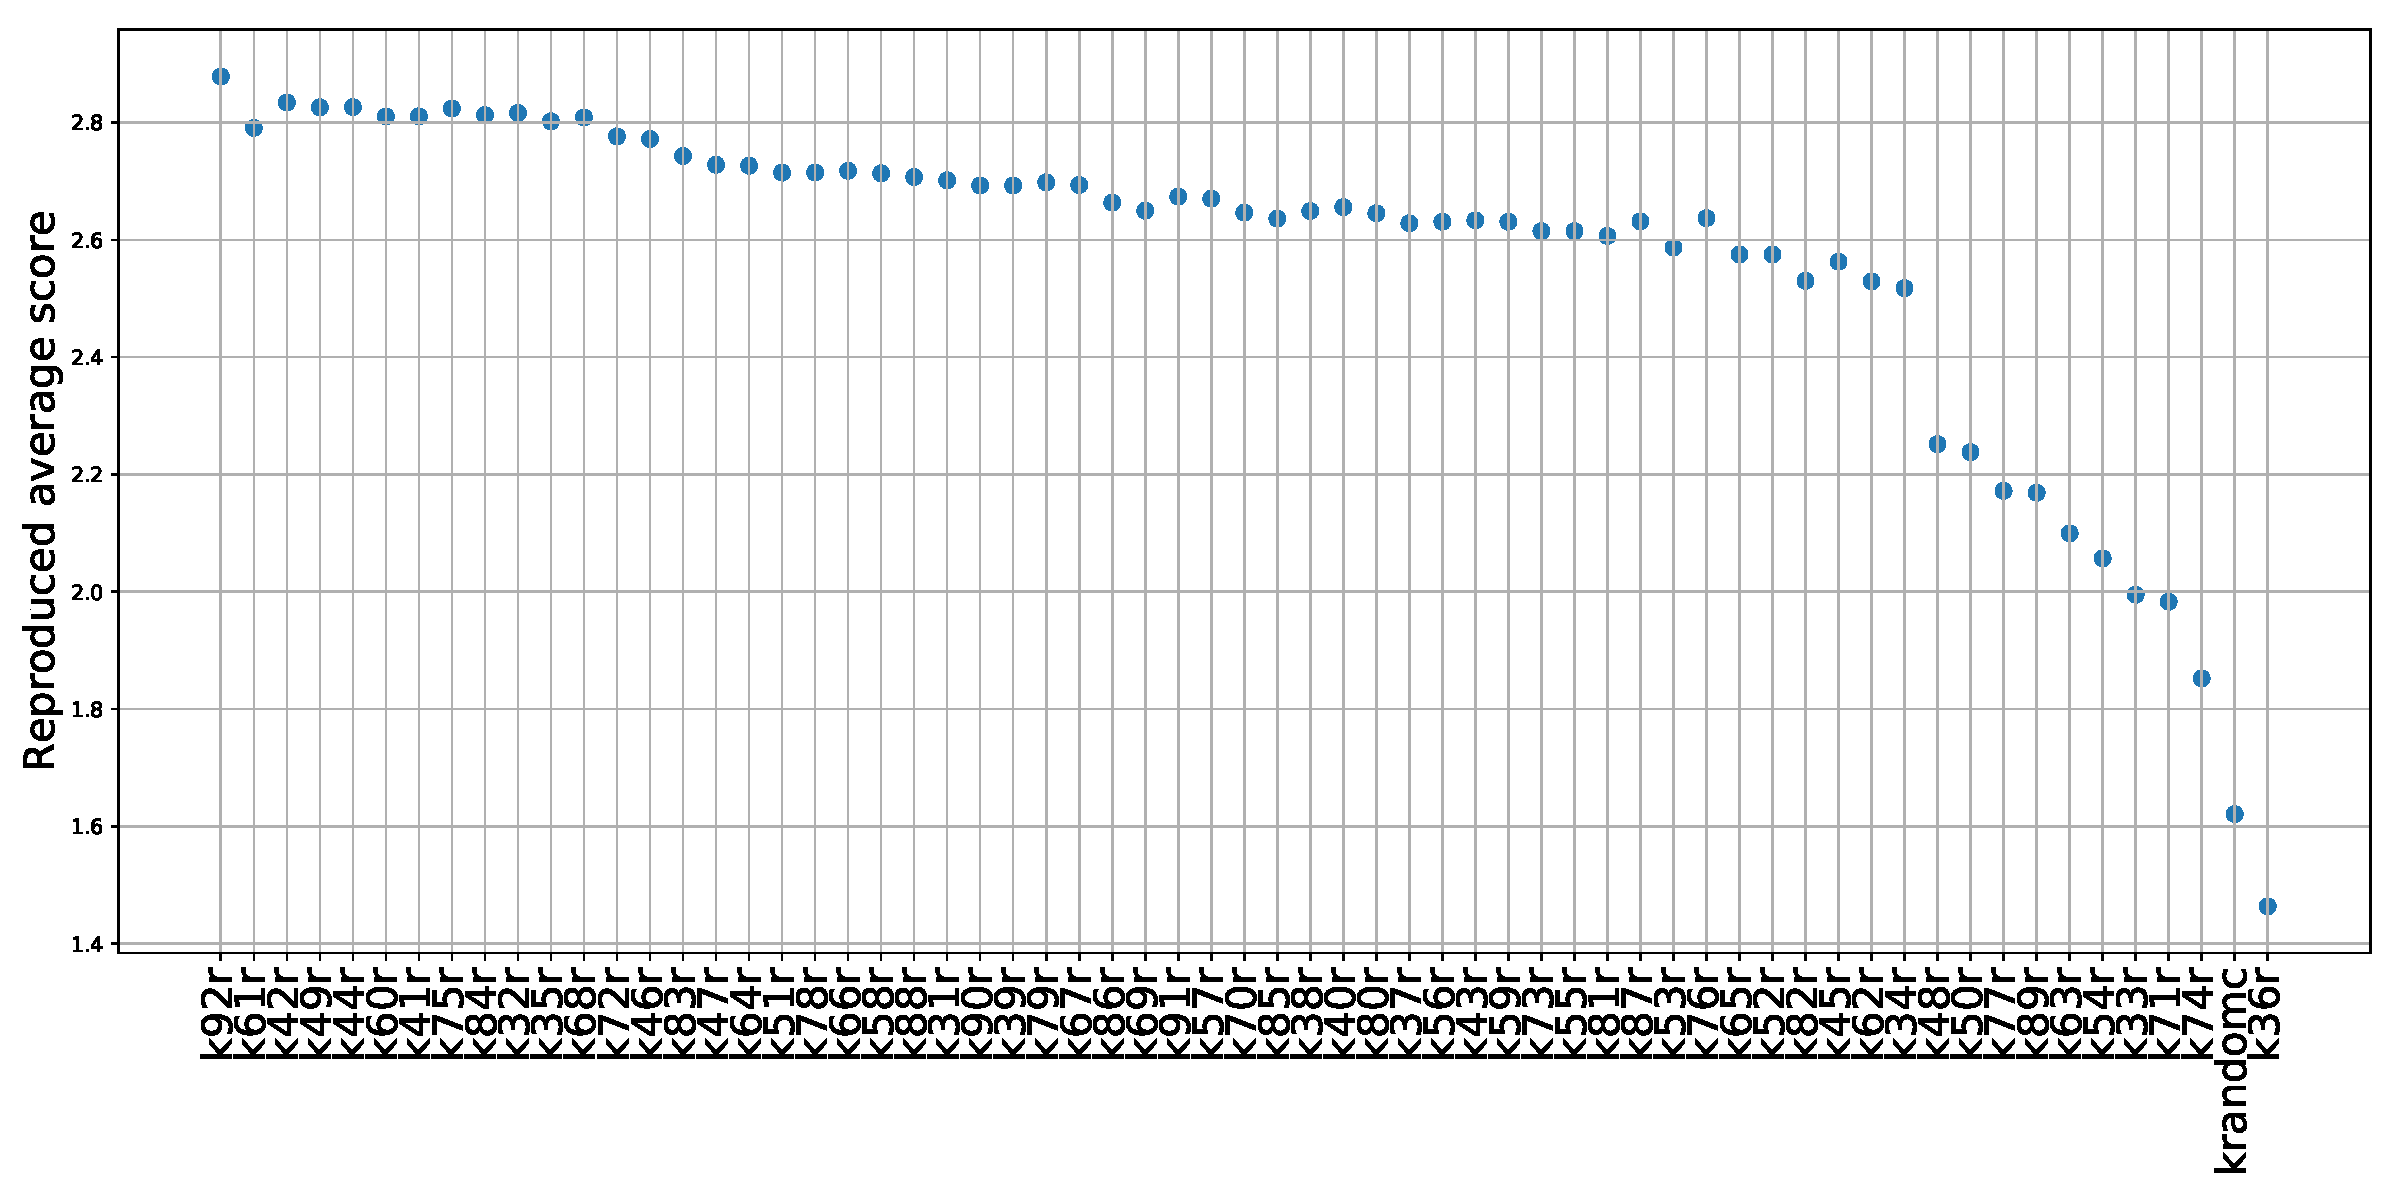
\includegraphics[width=.95\textwidth]{assets/original_tournament_scores.pdf}
        \caption{Average score per turn of each strategy.}
        \label{fig:original_tournament_scores}
    \end{subfigure}%
    ~
    \begin{subfigure}[t]{0.5\textwidth}
        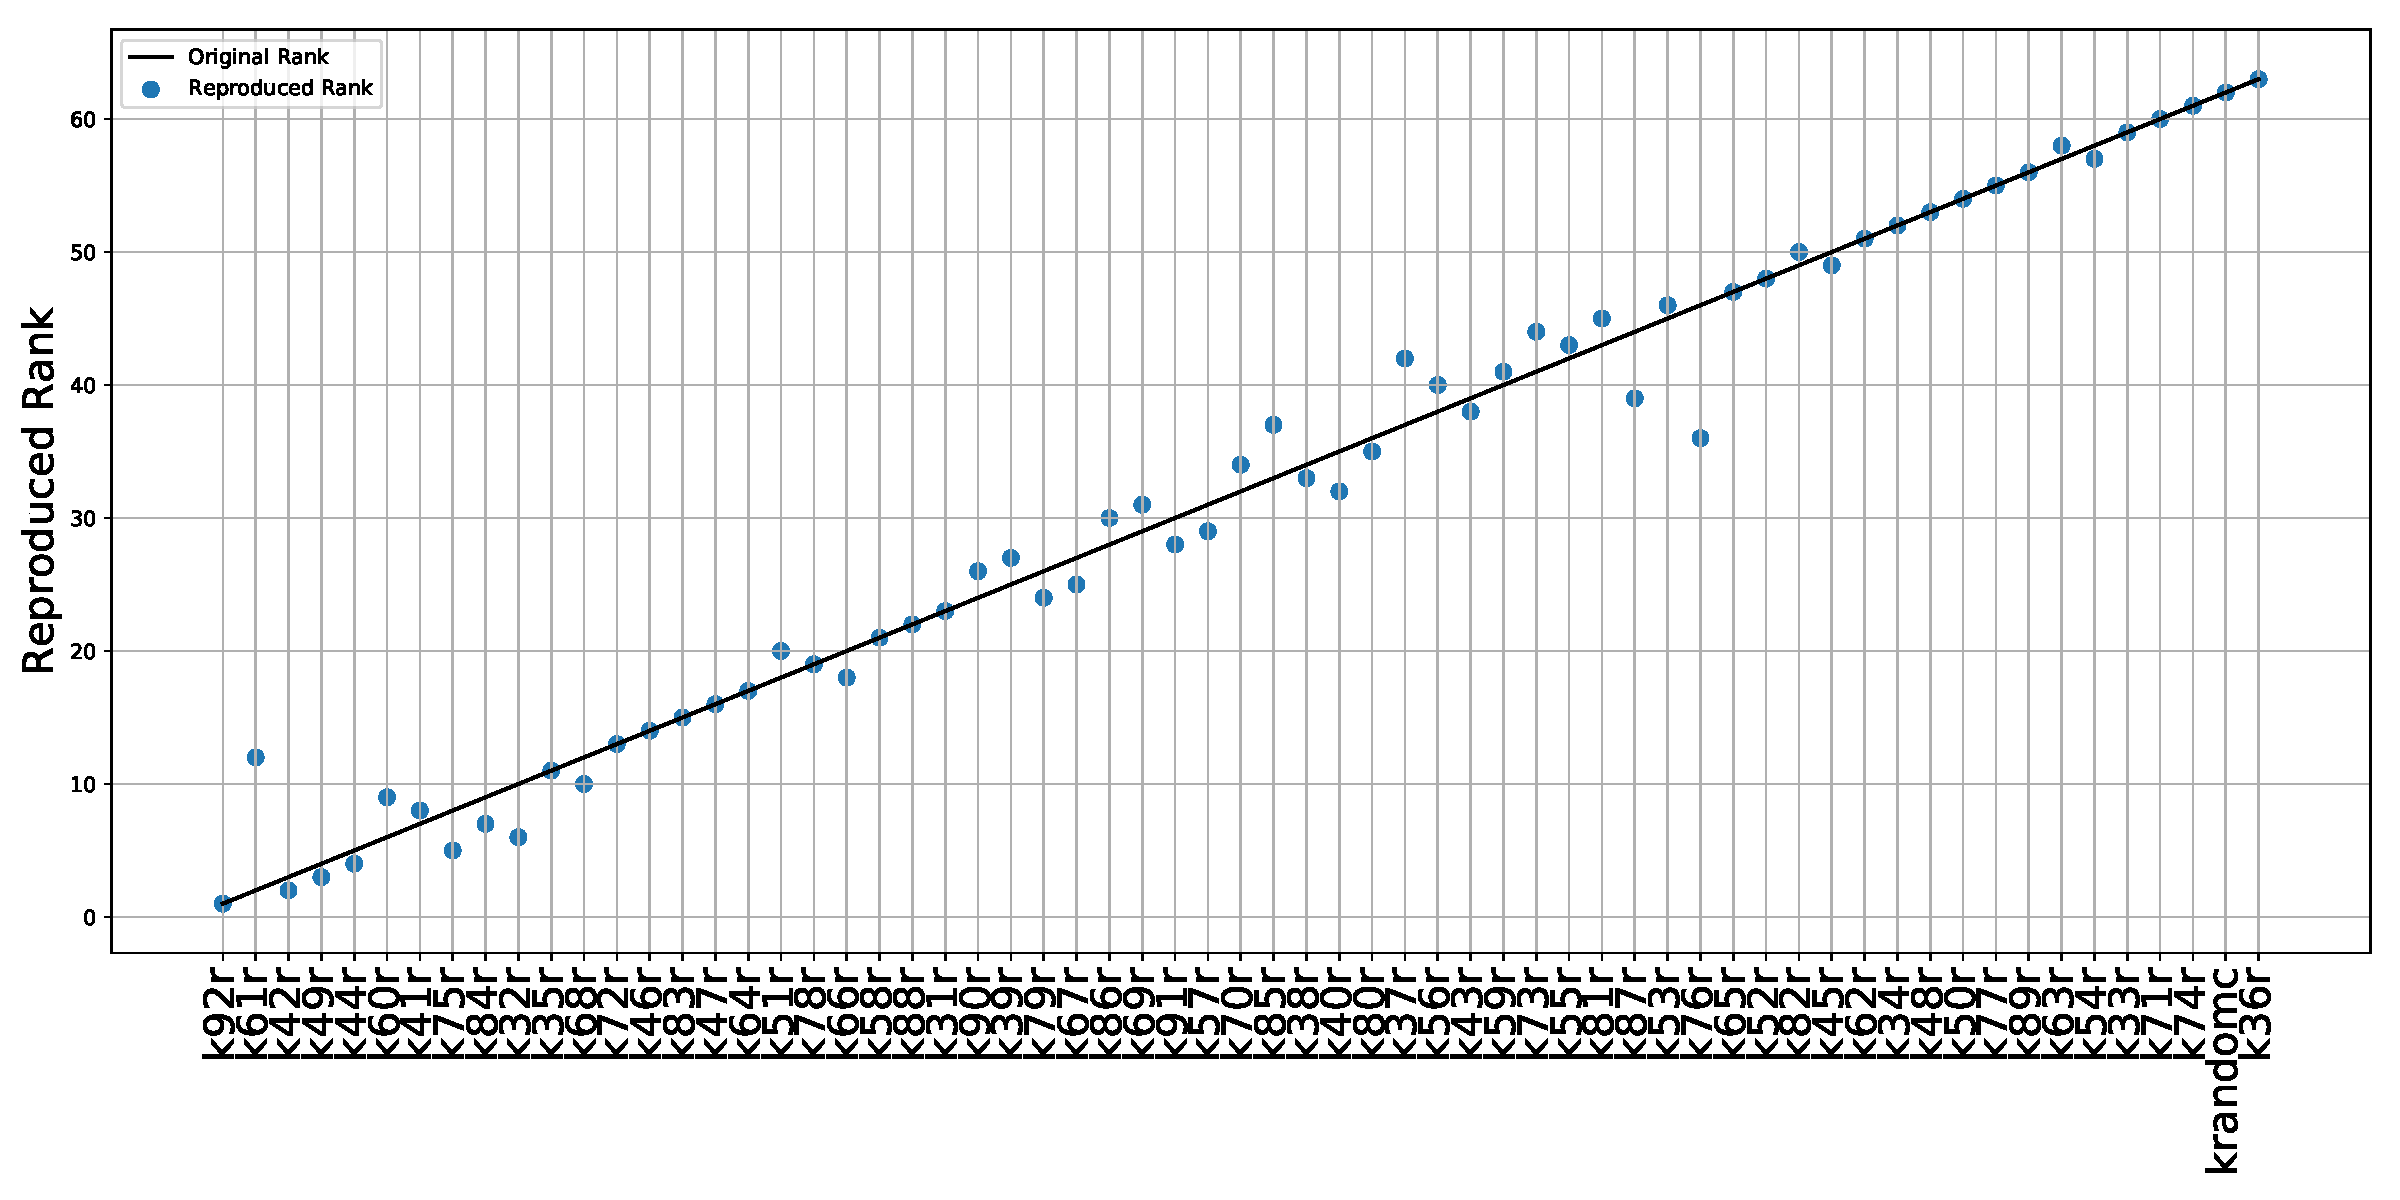
\includegraphics[width=.95\textwidth]{assets/original_tournament_rankings.pdf}
        \caption{Ranking of each strategy.}
        \label{fig:original_tournament_ranks}
    \end{subfigure}
    \caption{Replicated tournament with strategies ordered by original rank}
    \label{fig:replicated_tournament}
\end{figure}

The top 15 strategies in the reproduced tournament are shown in
Table~\ref{tbl:original_tournament_rankings}.

\begin{table}[!hbtp]
        \centering
        \begin{tabular}{llrrr}
\toprule
{} &                                 Author &  Scores &  Rank &  Original Rank \\
\midrule
k92r &                        Anatol Rapoport &  2.8786 &     1 &              1 \\
k61r &                       Danny C Champion &  2.7189 &    17 &              2 \\
k42r &                          Otto Borufsen &  2.8342 &     2 &              3 \\
k49r &                               Rob Cave &  2.8259 &     4 &              4 \\
k44r &                          William Adams &  2.8262 &     3 &              5 \\
k60r &           Jim Graaskamp and Ken Katzen &  2.8103 &     9 &              6 \\
k41r &                            Herb Weiner &  2.8104 &     8 &              7 \\
k75r &                      Paul D Harrington &  2.8240 &     5 &              8 \\
k84r &  T Nicolaus Tideman and Paula Chieruzz &  2.8126 &     7 &              9 \\
k32r &                       Charles Kluepfel &  2.8164 &     6 &             10 \\
k35r &                        Abraham Getzler &  2.8018 &    11 &             11 \\
k68r &                       Fransois Leyvraz &  2.8088 &    10 &             12 \\
k72r &                      Edward C White Jr &  2.7766 &    12 &             13 \\
k46r &                     Graham J Eatherley &  2.7724 &    13 &             14 \\
k83r &                           Paul E Black &  2.7427 &    14 &             15 \\
\bottomrule
\end{tabular}

        \caption{Top 15 strategies in the reproduced tournament}
        \label{tbl:original_tournament_rankings}
\end{table}

Whilst the results show an overall agreement with the original reported results,
a distinct outlier is \texttt{k61r}.
\texttt{k61r}: Is referred to as Champion: cooperates for the first 10
moves, plays tit for tat for the next fifteen and then will cooperate
unless: the other player defected on the previous move, the
other player cooperated less than 60\% and a random number between
0 and 1 is greater that the other player's cooperation rate. There is no
immediate explanation as to why this strategy does not perform as reported
in~\cite{Axelrod1980b}. Potential explanations include:

\begin{itemize}
    \item Stochastic variation not being sufficiently taken in to account
        in~\cite{Axelrod1980b}.
    \item A difference with how an older Fortran compiler would interpret the
        commands: this is not obvious though, the implemented version seems to
        interact as expected.
    \item An error in the reporting of~\cite{Axelrod1980b} which could include
        a modification of the source code.
\end{itemize}

Apart from this one outlier, the agreement between the original and the
reproduced tournament is significant. The main conclusions included for example
that Tit For Tat (\texttt{k92r}) once again wins the tournament. Furthermore,
the fact that high performing strategies are ``nice'' is also evident.
The overall cooperation rate of the tournament
is 0.750.
Figure~\ref{fig:replicated_cooperation_rates} shows the
cooperation rates of the tournament. It is clear that the high performing
strategies cooperate overall more often
(Figure~\ref{fig:original_tournament_cooperation_rates}). Also, looking at the
pairwise cooperation rates in
Figure~\ref{fig:original_tournament_pairwise_cooperation_rates} the high
performing strategies generally seems to cooperate with high performing
strategies. This underpins one of the main conclusions of~\cite{Axelrod1980b}
explaining the emergence of cooperation in competitive environments.

\begin{figure}[!hbtp]
    \begin{subfigure}{.6\textwidth}
        \centering
        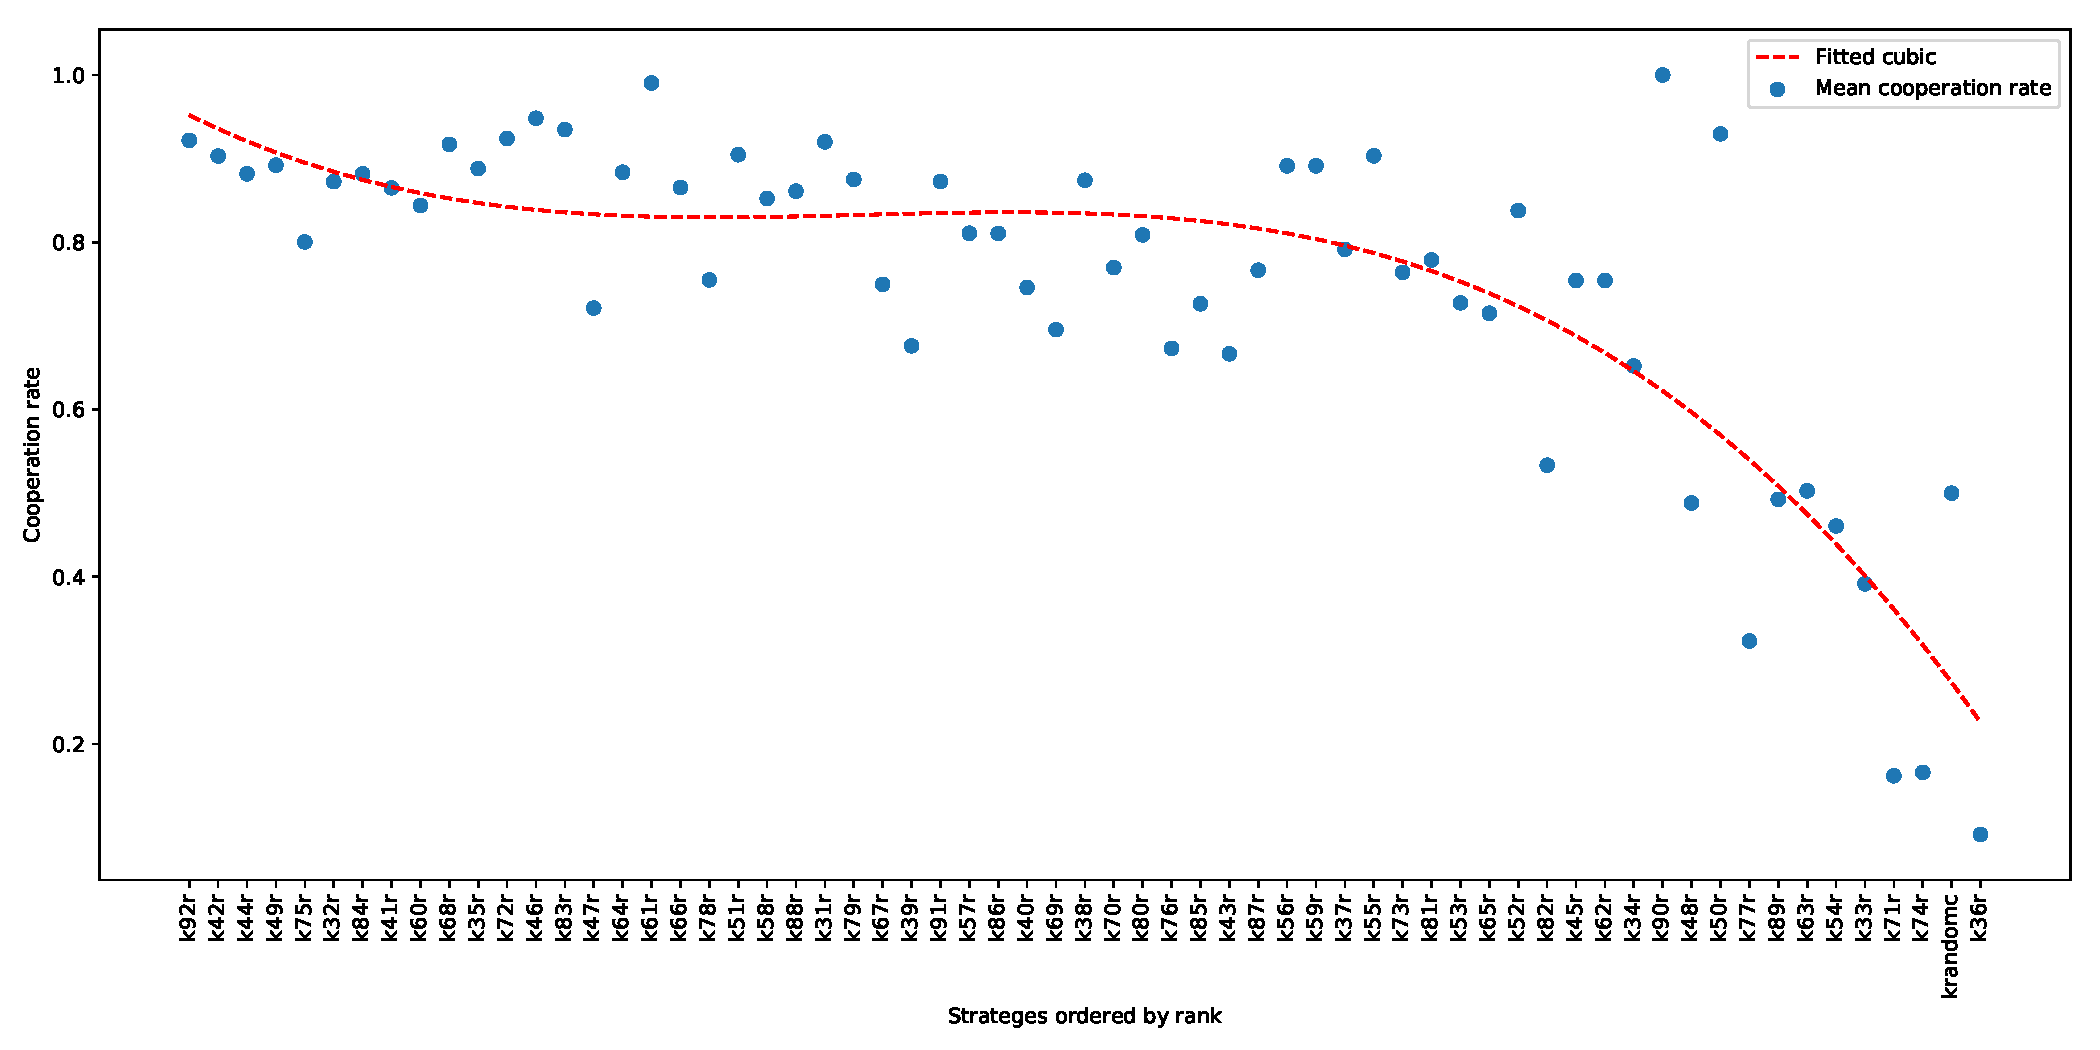
\includegraphics[width=.9\textwidth]{assets/original_tournament_cooperation_rate_versus_rank.pdf}
        \caption{Mean cooperation rates}
        \label{fig:original_tournament_cooperation_rate_versus_rank}
    \end{subfigure}%
    ~
    \begin{subfigure}{.4\textwidth}
        \centering
        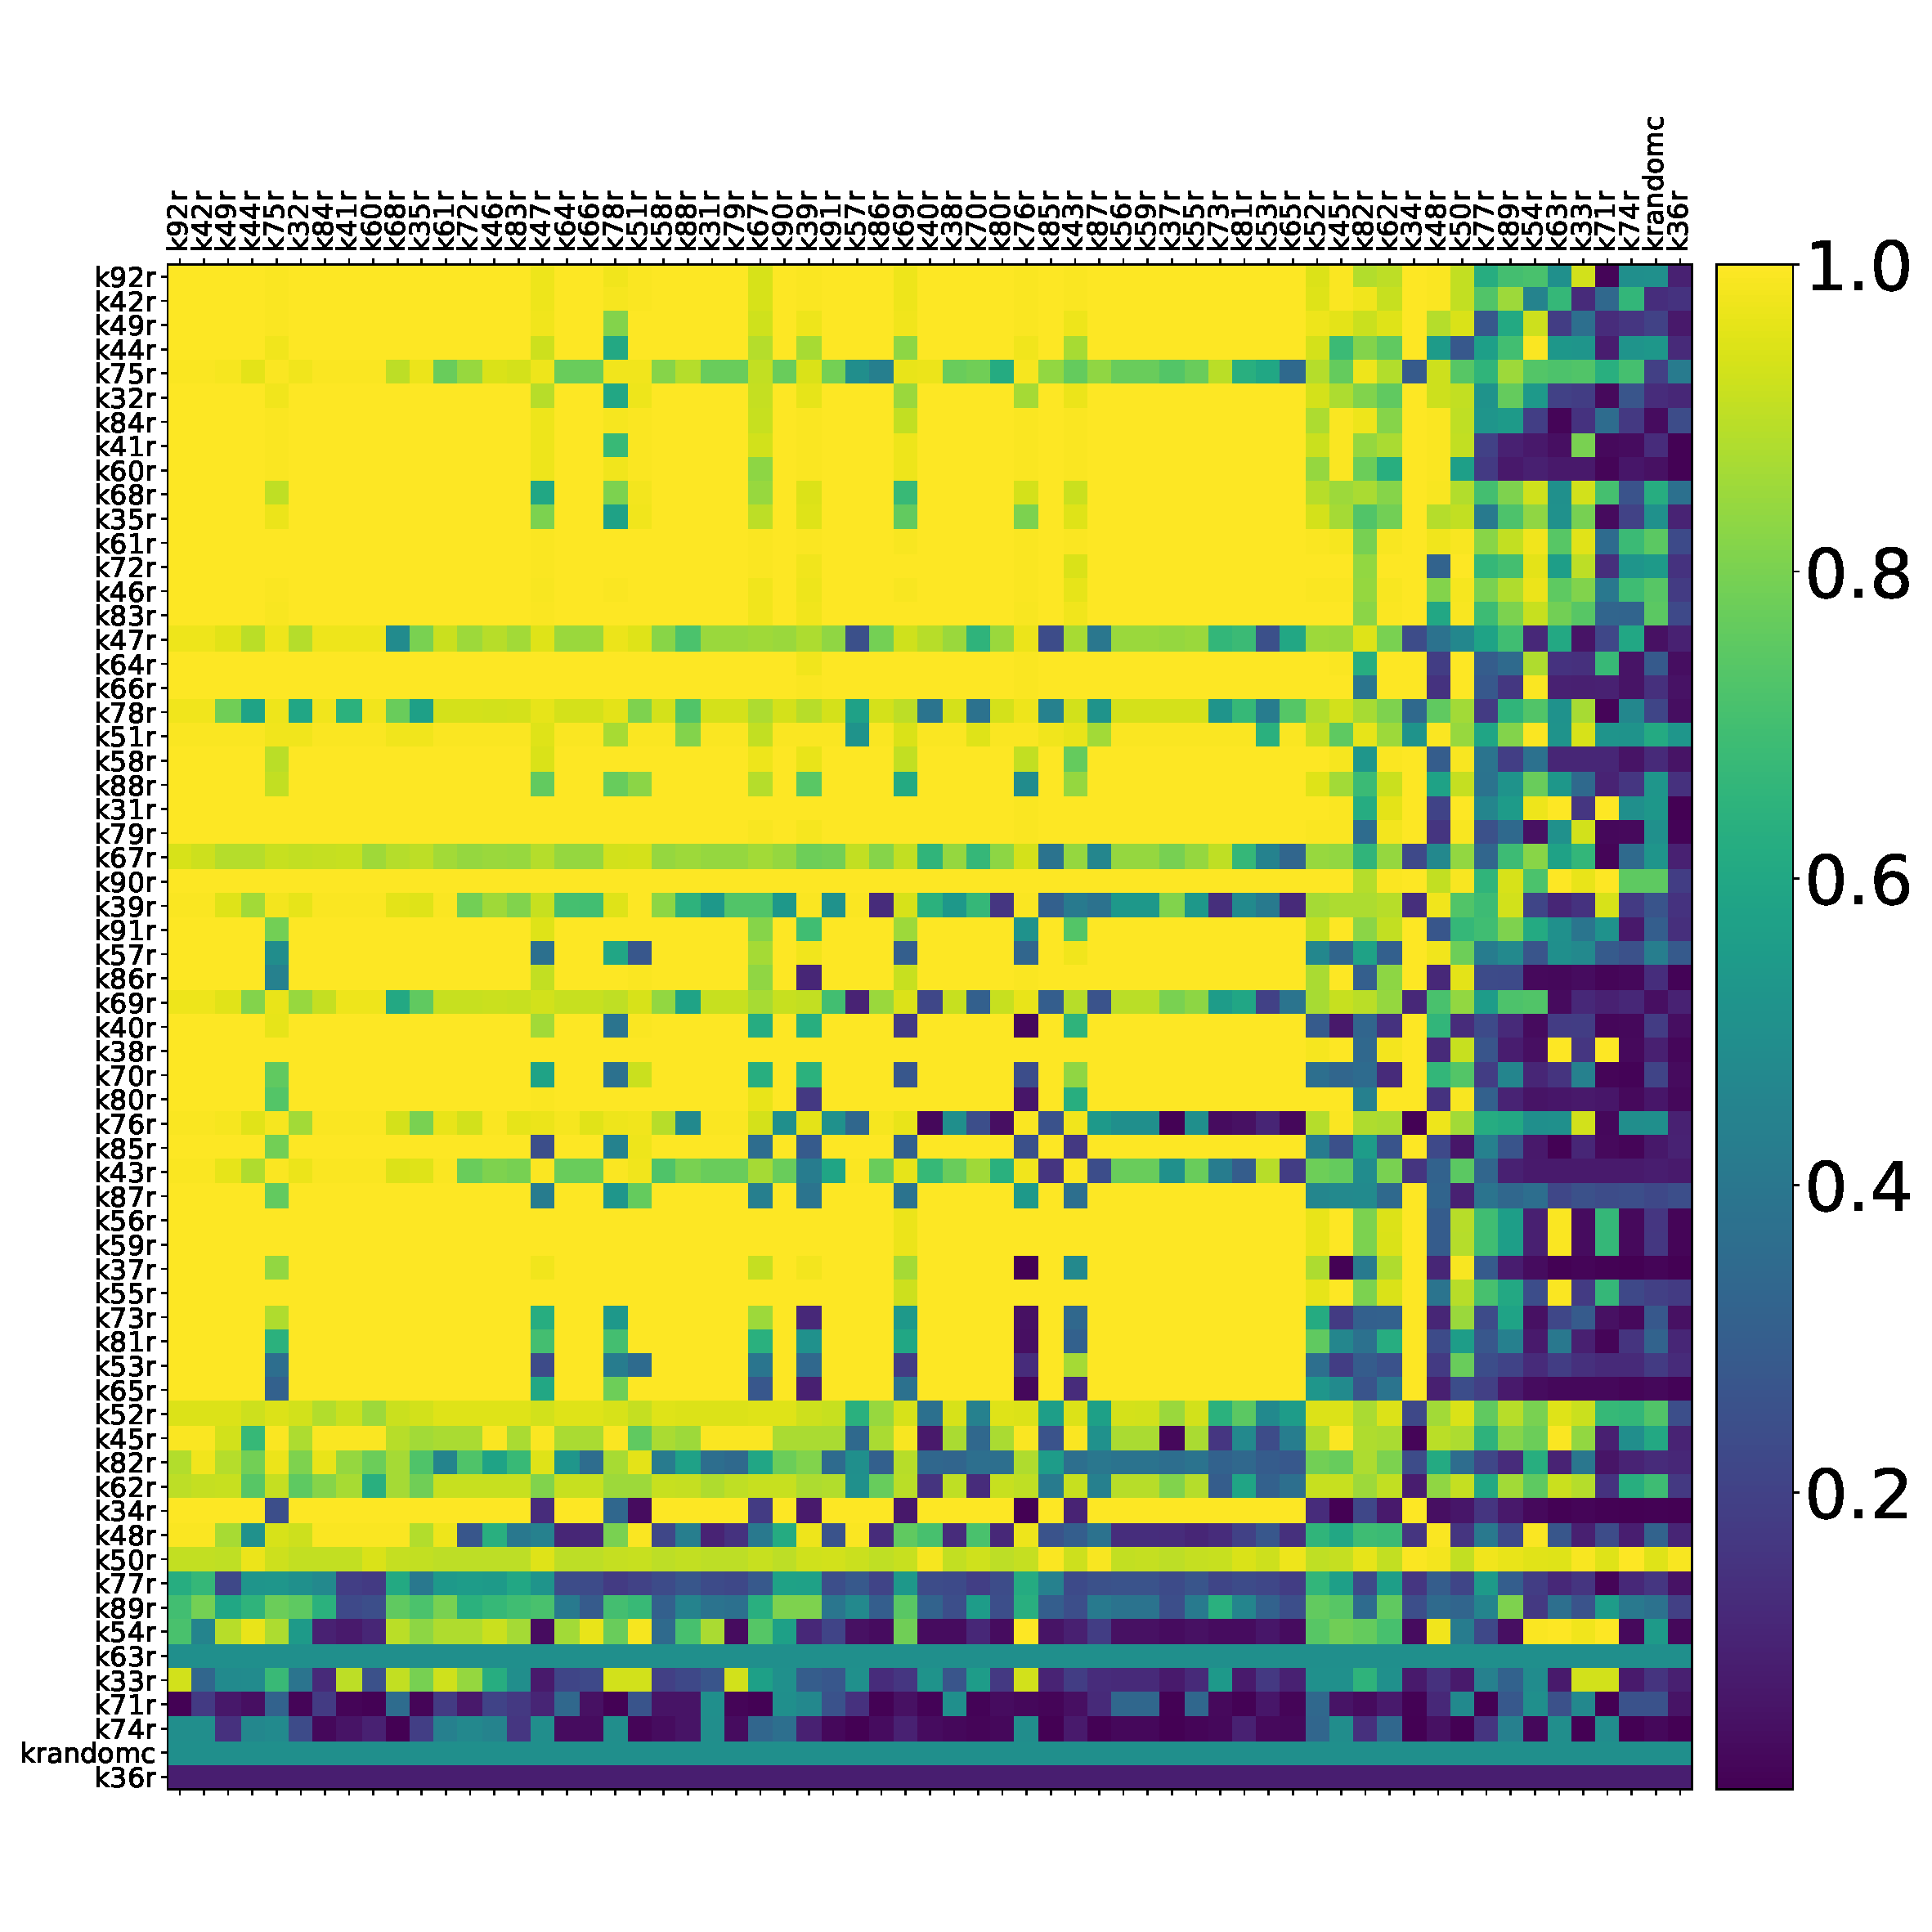
\includegraphics[width=.9\textwidth]{assets/original_tournament_pairwise_cooperation_rates.pdf}
        \caption{Cooperation rates between each pair of players}
        \label{fig:original_tournament_pairwise_cooperation_rates}
    \end{subfigure}
    \caption{Replicated tournament cooperation rates with strategies 
             ordered by original rank}
    \label{fig:replicated_cooperation_rates}
\end{figure}

For completeness in~\cite{Axelrod1980b}, a linear regression model is used to
identify 5 strategies, the scores against which are good predictors of the
overall performance. The reported \(R^2\) value is \(0.979\) (indicating 97\% of
variance accounted for by the model). The coefficients of this model are shown
in Table~\ref{tbl:original_tournament_representative_model}.

\begin{table}[!hbtp]
        \centering
        \begin{tabular}{lr}
\toprule
Strategies & Coefficients \\
\midrule
k69r & 0.202000 \\
k91r & 0.198000 \\
k40r & 0.110000 \\
k76r & 0.072000 \\
k67r & 0.086000 \\
Intercept & 0.795000 \\
\bottomrule
\end{tabular}

        \caption{Linear model described in~\cite{Axelrod1980b} with
             \(R^2=\protect0.7508\)}
        \label{tbl:original_tournament_representative_model}
\end{table}

Given the discrepancy in results shown in
Figure~\ref{fig:replicated_tournament} and
Table~\ref{tbl:original_tournament_rankings} it is not surprising to see that
this model no longer performs as well with
\(R^2=0.7508\).

Fitting a new model to the same 5 strategies gives the coefficients shown in
Table~\ref{tbl:original_tournament_predictive_with_axelrod_5_model} with
\(R^2=0.9440\)

\begin{table}[!hbtp]
        \centering
        \begin{tabular}{lrll}
\toprule
Strategies & Coefficients & $p$-value & $F$-value \\
\midrule
k69r & 0.098640 & 0.000000 & 43.976036 \\
k91r & 0.207380 & 0.000000 & 56.667196 \\
k40r & 0.206440 & 0.000000 & 78.191831 \\
k76r & 0.059930 & 0.025992 & 5.207451 \\
k67r & 0.123740 & 0.000002 & 27.893148 \\
Intercept & 0.768410 & NA & NA \\
\bottomrule
\end{tabular}

        \caption{Linear model fitted to the same 5 strategies described
                 in~\cite{Axelrod1980b} with
             \(R^2=\protect0.9440\)}
        \label{tbl:original_tournament_predictive_with_axelrod_5_model}
\end{table}

Using recursive feature elimination
% TODO Include a text book reference
It is possible to select the features (strategies) that give the best prediction
for a given number of features. The \(R^2\) versus the number of features is
shown in
Figure~\ref{fig:original_tournament_r_squared_versus_number_of_features}.

\begin{figure}[!hbtp]
    \centering
    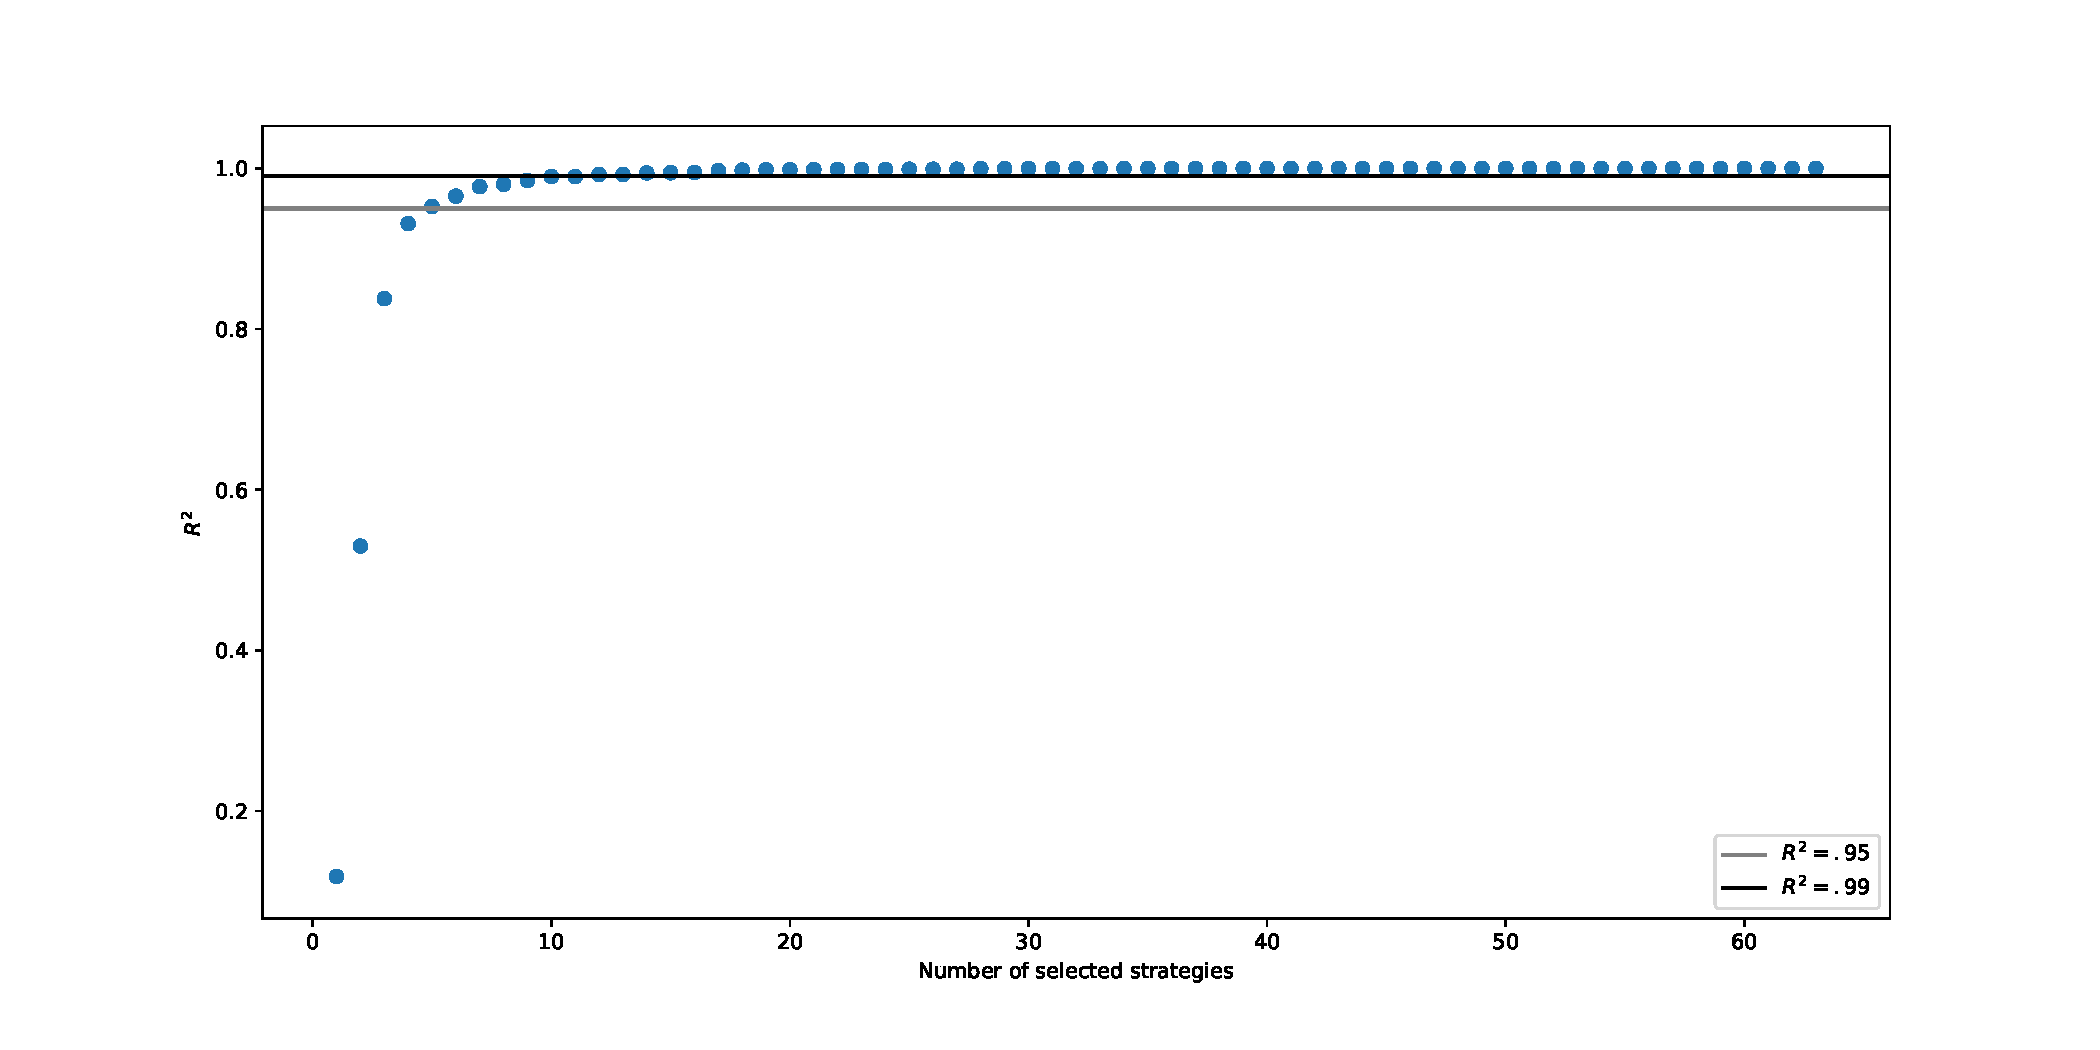
\includegraphics[width=.8\textwidth]{assets/original_tournament_r_squared_versus_number_of_features.pdf}
    \caption{\(R^2\) for models obtained using recursive feature elimination.}
    \label{fig:original_tournament_r_squared_versus_number_of_features}
\end{figure}


Tables~\ref{tbl:original_tournament_predictive_5_model}
and~\ref{tbl:original_tournament_predictive_12_model} show the coefficients for
linear models fitted to 5 and 12 strategies with
\(R^2=0.9440\) and
\(R^2=0.9930\)
respectively (12 strategies is the smallest number of strategies for which
\(R^2>95\)).


\begin{table}[!hbtp]
        \centering
        \begin{tabular}{lrll}
\toprule
Strategies &  Coefficients &    $p$-value & $F$-value \\
\midrule
      k55r &         0.191 &  5.20963e-08 &   38.5403 \\
      k73r &         0.165 &  2.42582e-11 &   66.4276 \\
      k82r &         0.134 &  1.80697e-06 &   27.8953 \\
      k84r &         0.092 &  6.31455e-18 &   147.489 \\
      k92r &         0.188 &  2.68503e-13 &    86.435 \\
 Intercept &         0.520 &           NA &        NA \\
\bottomrule
\end{tabular}

        \caption{Linear model best fitted to 5 strategies in the reproduced tournament
                 with
             \(R^2=\protect0.9440\)}
        \label{tbl:original_tournament_predictive_5_model}
\end{table}

\begin{table}[!hbtp]
        \centering
        \begin{tabular}{lrll}
\toprule
Strategies &  Coefficients &    $p$-value & $F$-value \\
\midrule
      k31r &         0.166 &  5.15065e-05 &   18.9782 \\
      k34r &         0.081 &  1.39931e-08 &   42.8242 \\
      k51r &         0.230 &   0.00357868 &    9.1841 \\
      k52r &         0.116 &     0.572461 &   0.32205 \\
      k56r &        -1.695 &   1.2278e-09 &   51.2719 \\
      k59r &         1.729 &   1.2399e-09 &   51.2364 \\
      k64r &        -0.150 &  2.41824e-14 &   98.4147 \\
      k79r &         0.121 &  2.36814e-14 &   98.5231 \\
      k82r &         0.120 &  1.08815e-06 &   29.3393 \\
      k84r &         0.220 &  9.37609e-18 &   144.822 \\
      k88r &         0.112 &   1.8614e-15 &   112.266 \\
      k91r &         0.066 &  2.50396e-10 &   57.1748 \\
 Intercept &        -0.485 &           NA &        NA \\
\bottomrule
\end{tabular}

        \caption{Linear model best fitted to 12 strategies in the reproduced tournament
                 with
             \(R^2=\protect0.9930\)}
        \label{tbl:original_tournament_predictive_12_model}
\end{table}

The predictions of these models are shown in
Figure~\ref{fig:original_tournament_predictive_score_models}.

\begin{figure}[!hbtp]
    \centering
    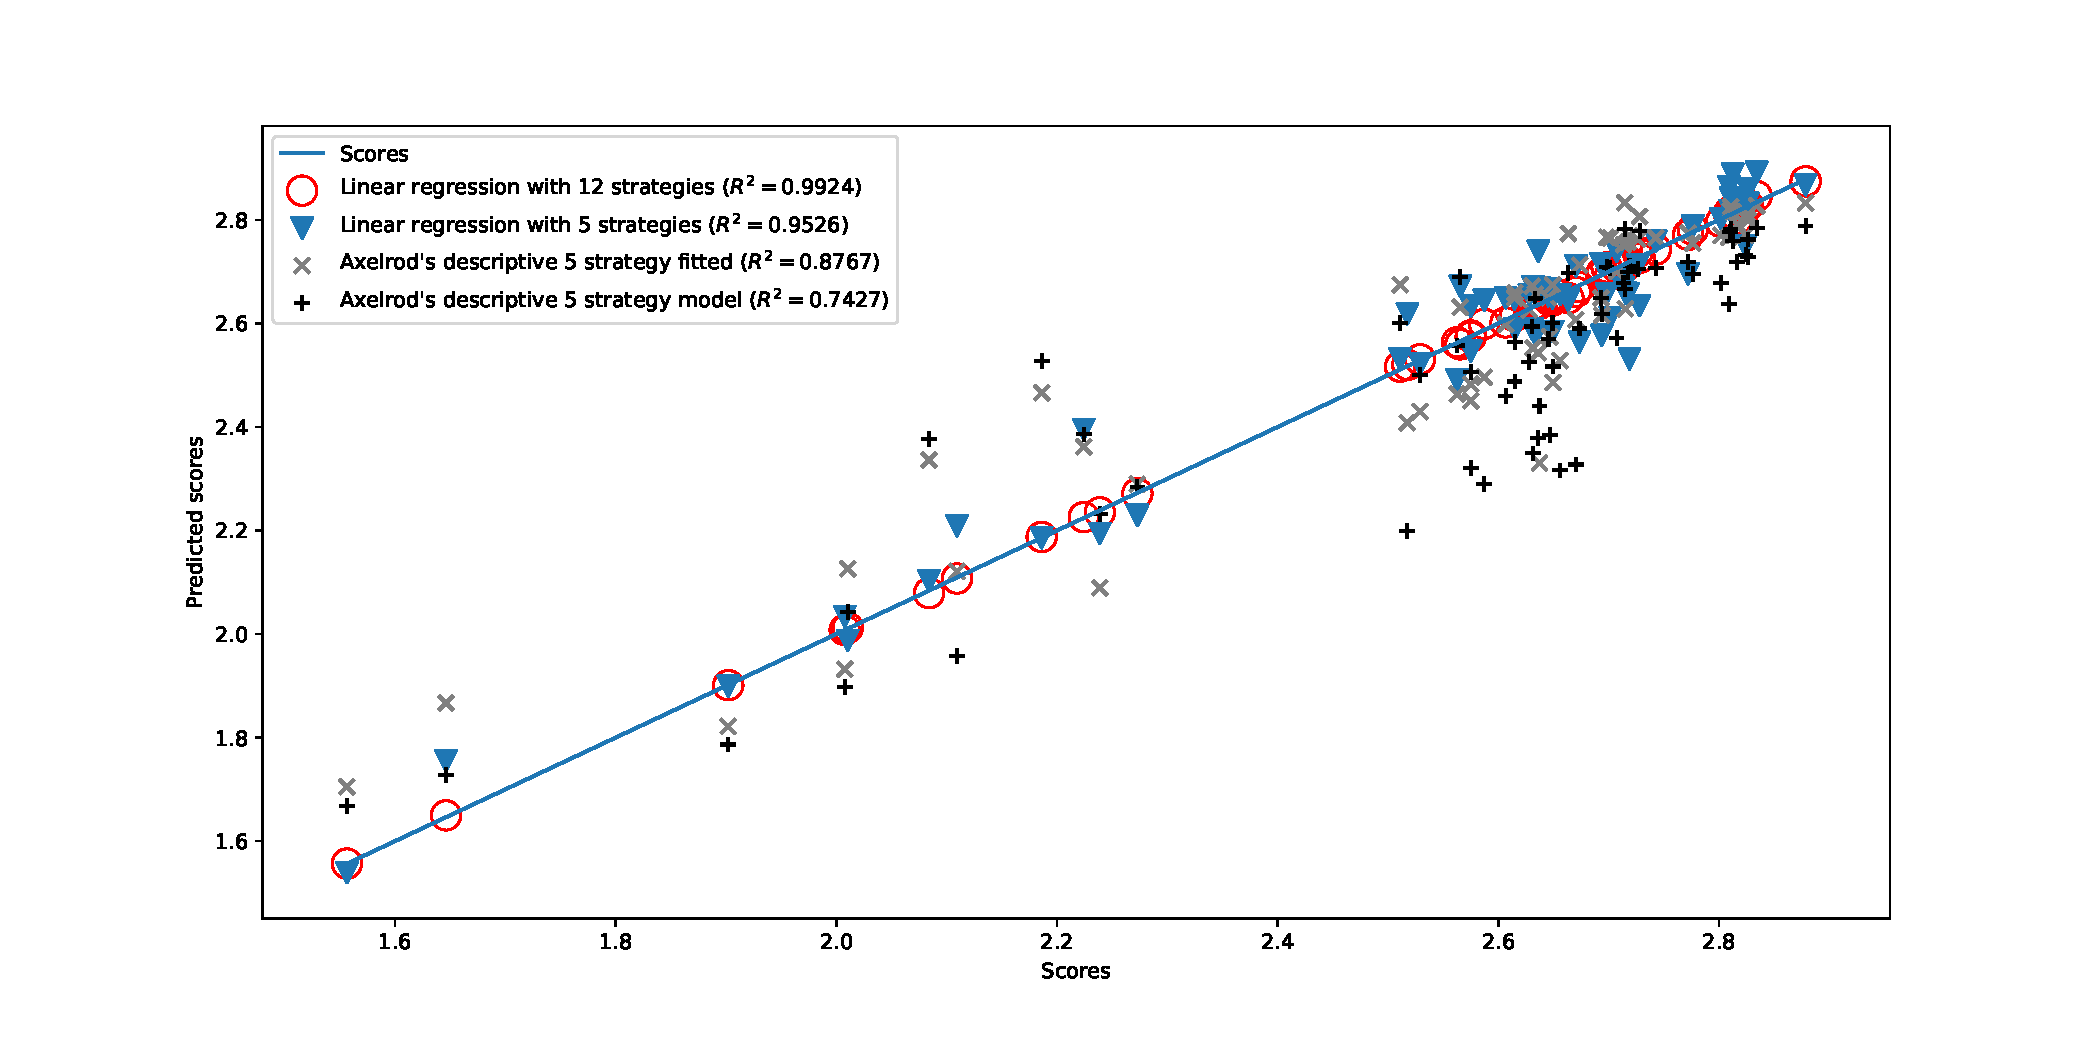
\includegraphics[width=.9\textwidth]{assets/original_tournament_predictive_score_models.pdf}
    \caption{Predicting the performance of strategies using the 4 models
             discussed}
    \label{fig:original_tournament_predictive_score_models}
\end{figure}

It is clear that the effectiveness of the predictive models with 5 strategies is
low for the cluster of highly performing strategies (with a score great than
2.5). To be able to obtain a good model even for high performing strategies 12
seem to provide a good predictive model. These predictive models will be
revisited in Section~\ref{sec:trained_strategies}.

\section{Revisiting the tournament}\label{sec:revisiting}

In this section, the tournament of~\cite{Axelrod1980b} will be revisited.
Indeed, a large amount of research has gone on since Axelrod's original work
which include for example training of strategies using reinforcement
learning~\cite{Harper2017}
but also the discovery of Zero Determinant strategies~\cite{Press2012}. This
section aims to measure how well these strategies would have faired and
\textbf{if} any of the original insights and conclusions would differ.

\subsection{Running with an extra invitation}\label{sec:extra_strategy}

\subsubsection{Known strategies}

The tournament is run with every strategy of the Axelrod library.
% TODO Cite properly
% TODO Point at appendix
Every tournament (corresponding to each strategy) was run
for 4000repetitions.
Table~\ref{tbl:original_tournament_with_extra_strategy_summary} shows the top
ranking strategies.

\begin{table}[!hbtp]
        \tiny
        \centering
        \begin{tabular}{lrrl}
\toprule
 & Mean Score & Rank & Winner \\
Name &  &  &  \\
\midrule
Adaptive Tit For Tat: 0.5 & 2.876 & 2 & k92r \\
GTFT: 0.33 & 2.846 & 3 & k92r \\
Omega TFT: 3, 8 & 2.859 & 3 & k92r \\
Firm But Fair & 2.861 & 3 & k92r \\
ZD-GTFT-2: 0.25, 0.5 & 2.868 & 3 & k92r \\
Resurrection & 2.867 & 3 & k92r \\
Meta Majority: 213 players & 2.860 & 3 & k92r \\
Meta Majority Finite Memory: 79 players & 2.856 & 3 & k92r \\
Meta Majority Long Memory: 134 players & 2.856 & 3 & k92r \\
Soft Joss: 0.9 & 2.871 & 3 & k92r \\
Forgiving Tit For Tat & 2.854 & 3 & k92r \\
Original Gradual & 2.857 & 3 & k92r \\
Meta Majority Memory One: 36 players & 2.838 & 4 & k92r \\
PSO Gambler 2\_2\_2 Noise 05 & 2.840 & 4 & k92r \\
Gradual & 2.831 & 7 & k92r \\
First by Stein and Rapoport: 0.05: (D, D) & 2.827 & 8 & k92r \\
Spiteful Tit For Tat & 2.826 & 8 & k92r \\
GrudgerAlternator & 2.825 & 8 & k92r \\
EugineNier: (D,) & 2.815 & 10 & k92r \\
First by Shubik & 2.791 & 13 & k92r \\
\bottomrule
\end{tabular}

        \caption{Performance of extra strategy in Axelrod's original tournament}
        \label{tbl:original_tournament_with_extra_strategy_summary}
\end{table}

Figure~\ref{fig:original_tournament_with_extra_strategy_ranks_vs_library_ranks}
shows the rank of the extra strategy against it's rank in the library
tournament.

\begin{figure}[!hbtp]
    \centering
    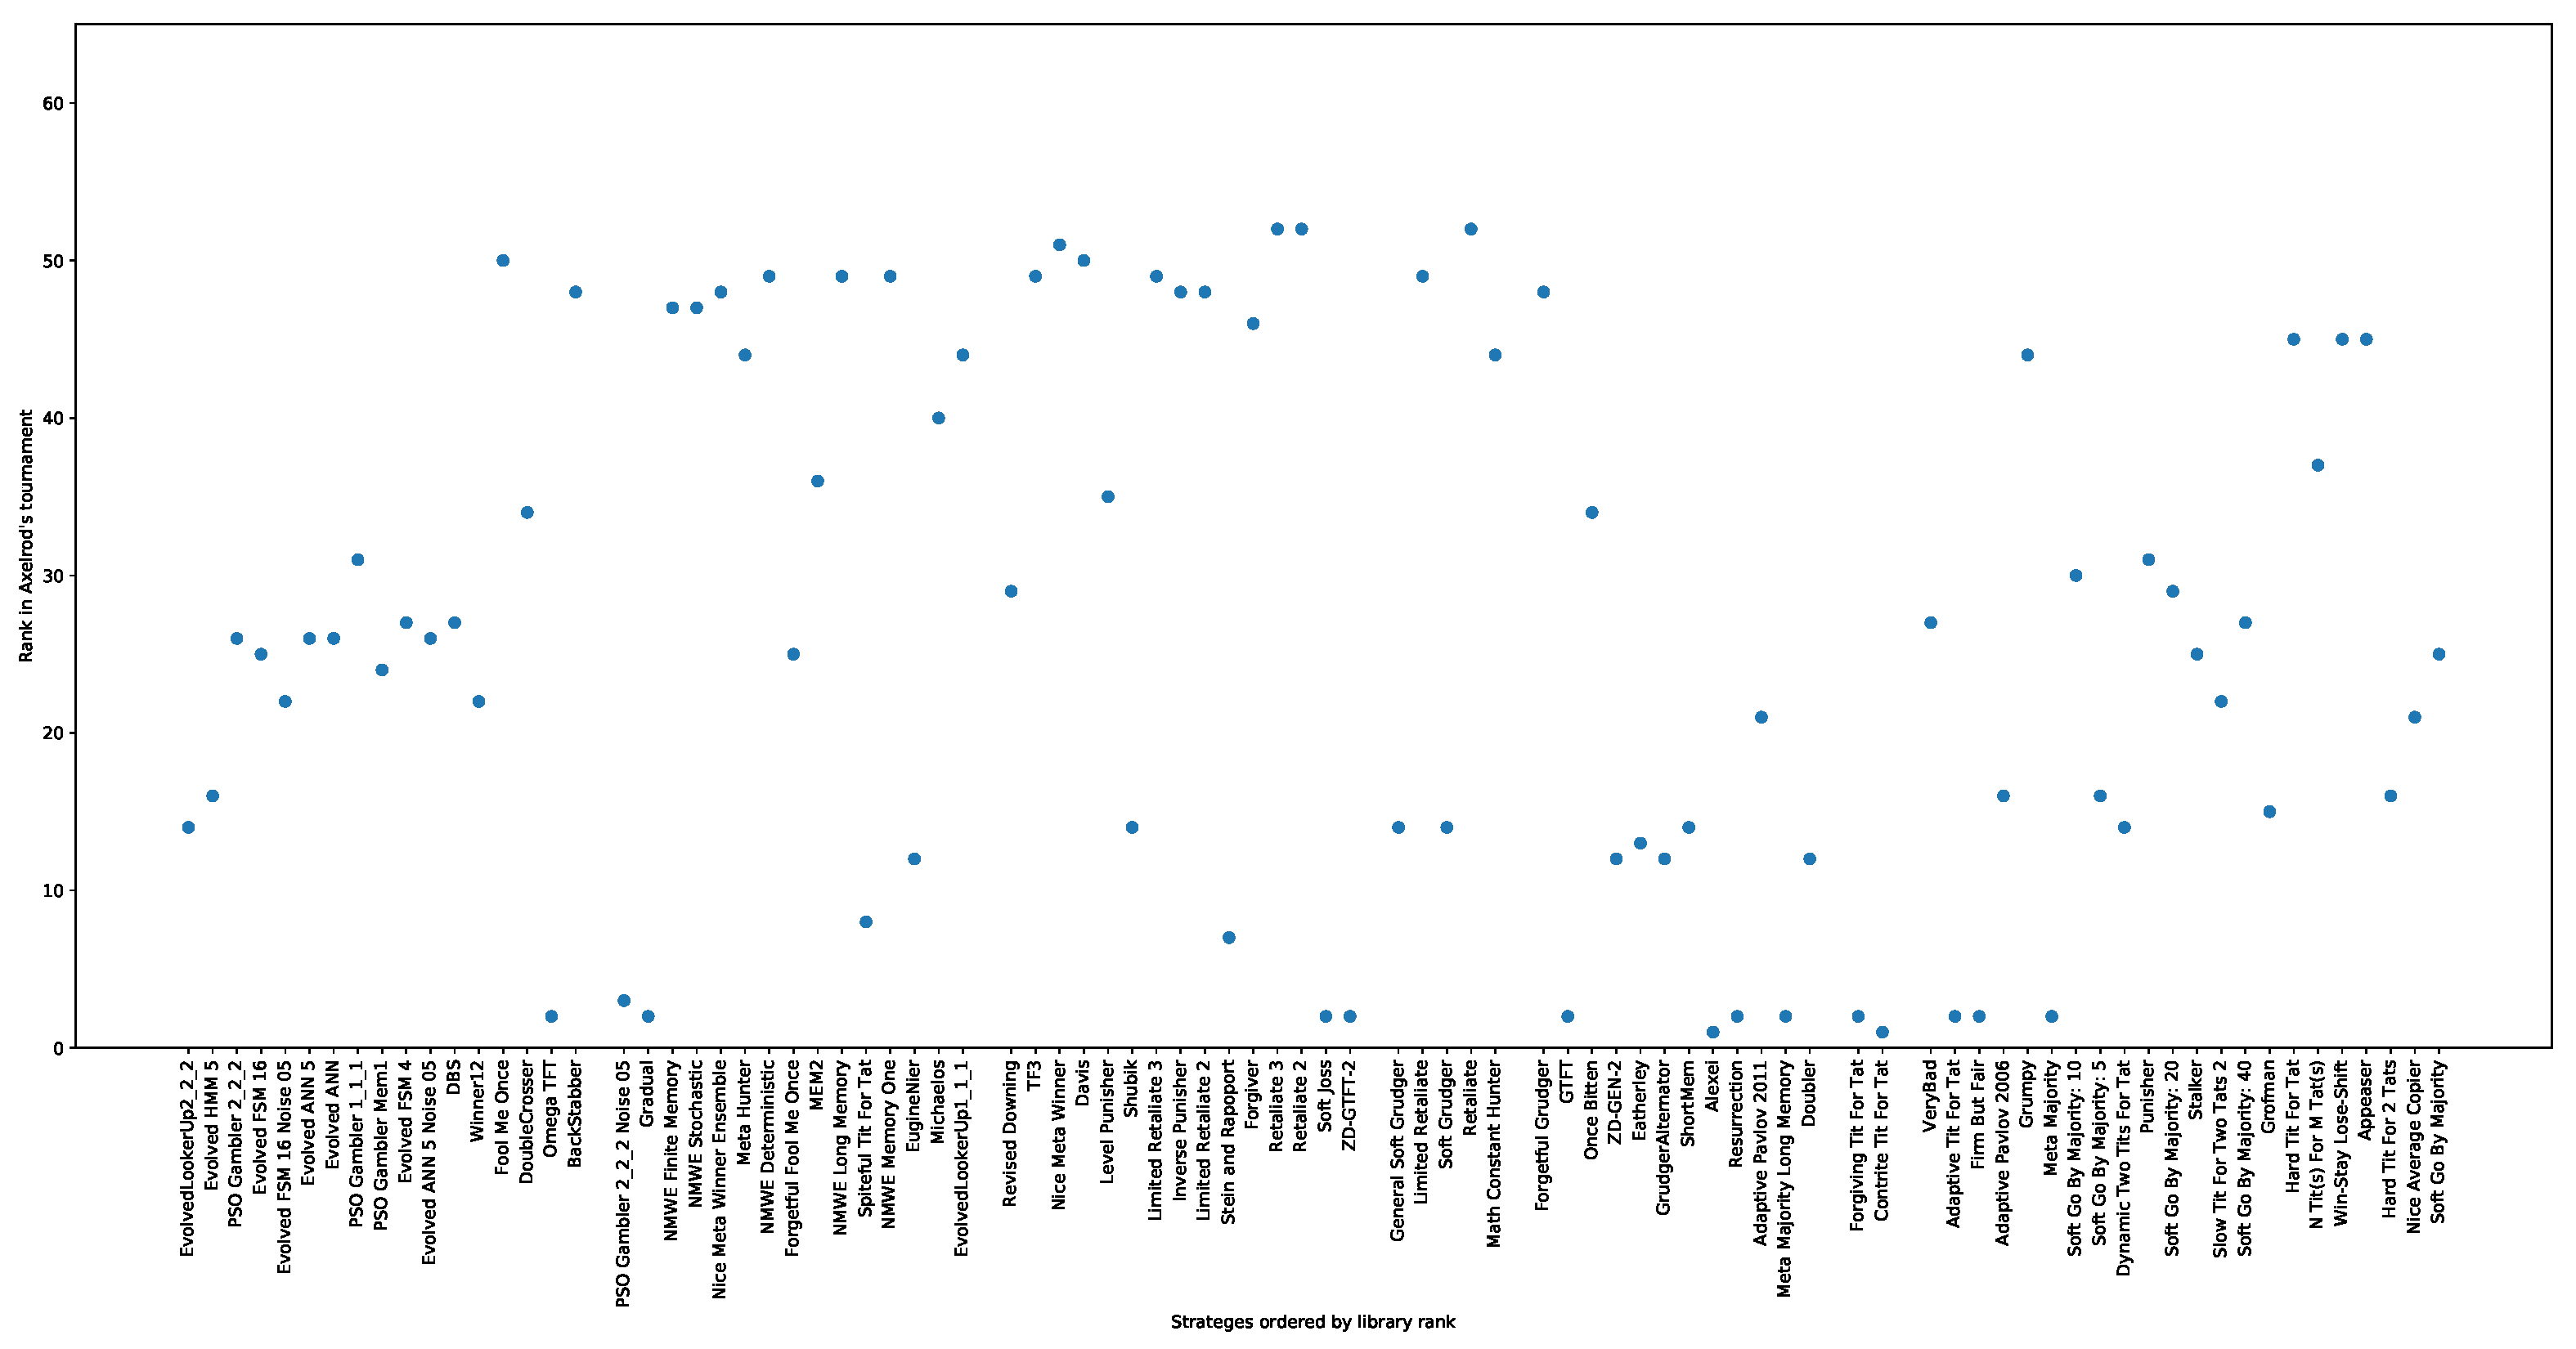
\includegraphics[width=.8\textwidth]{assets/original_tournament_with_extra_strategy_ranks_vs_library_ranks.pdf}
    \caption{Ranks of extra strategy}
    \label{fig:original_tournament_with_extra_strategy_ranks_vs_library_ranks}
\end{figure}

\subsubsection{Trained strategies}\label{sec:trained_strategies}

Using the various strategy sets and weights from the previous regression
analysis
% TODO Improve how this points and refers to training
it is possible to train strategies to compete in the tournament.
% TODO Add details about training (software + algorithm): also include a diagram
% about process (mutation and crossover)
Figure~\ref{fig:training_data_max_score} show the mean utility of the strategies
trained for this work. The strategies trained are 10 state Finite State
machines.
% TODO Include references.
% TODO Draw final fsm ones.

\begin{figure}[!hbtp]
    \centering
    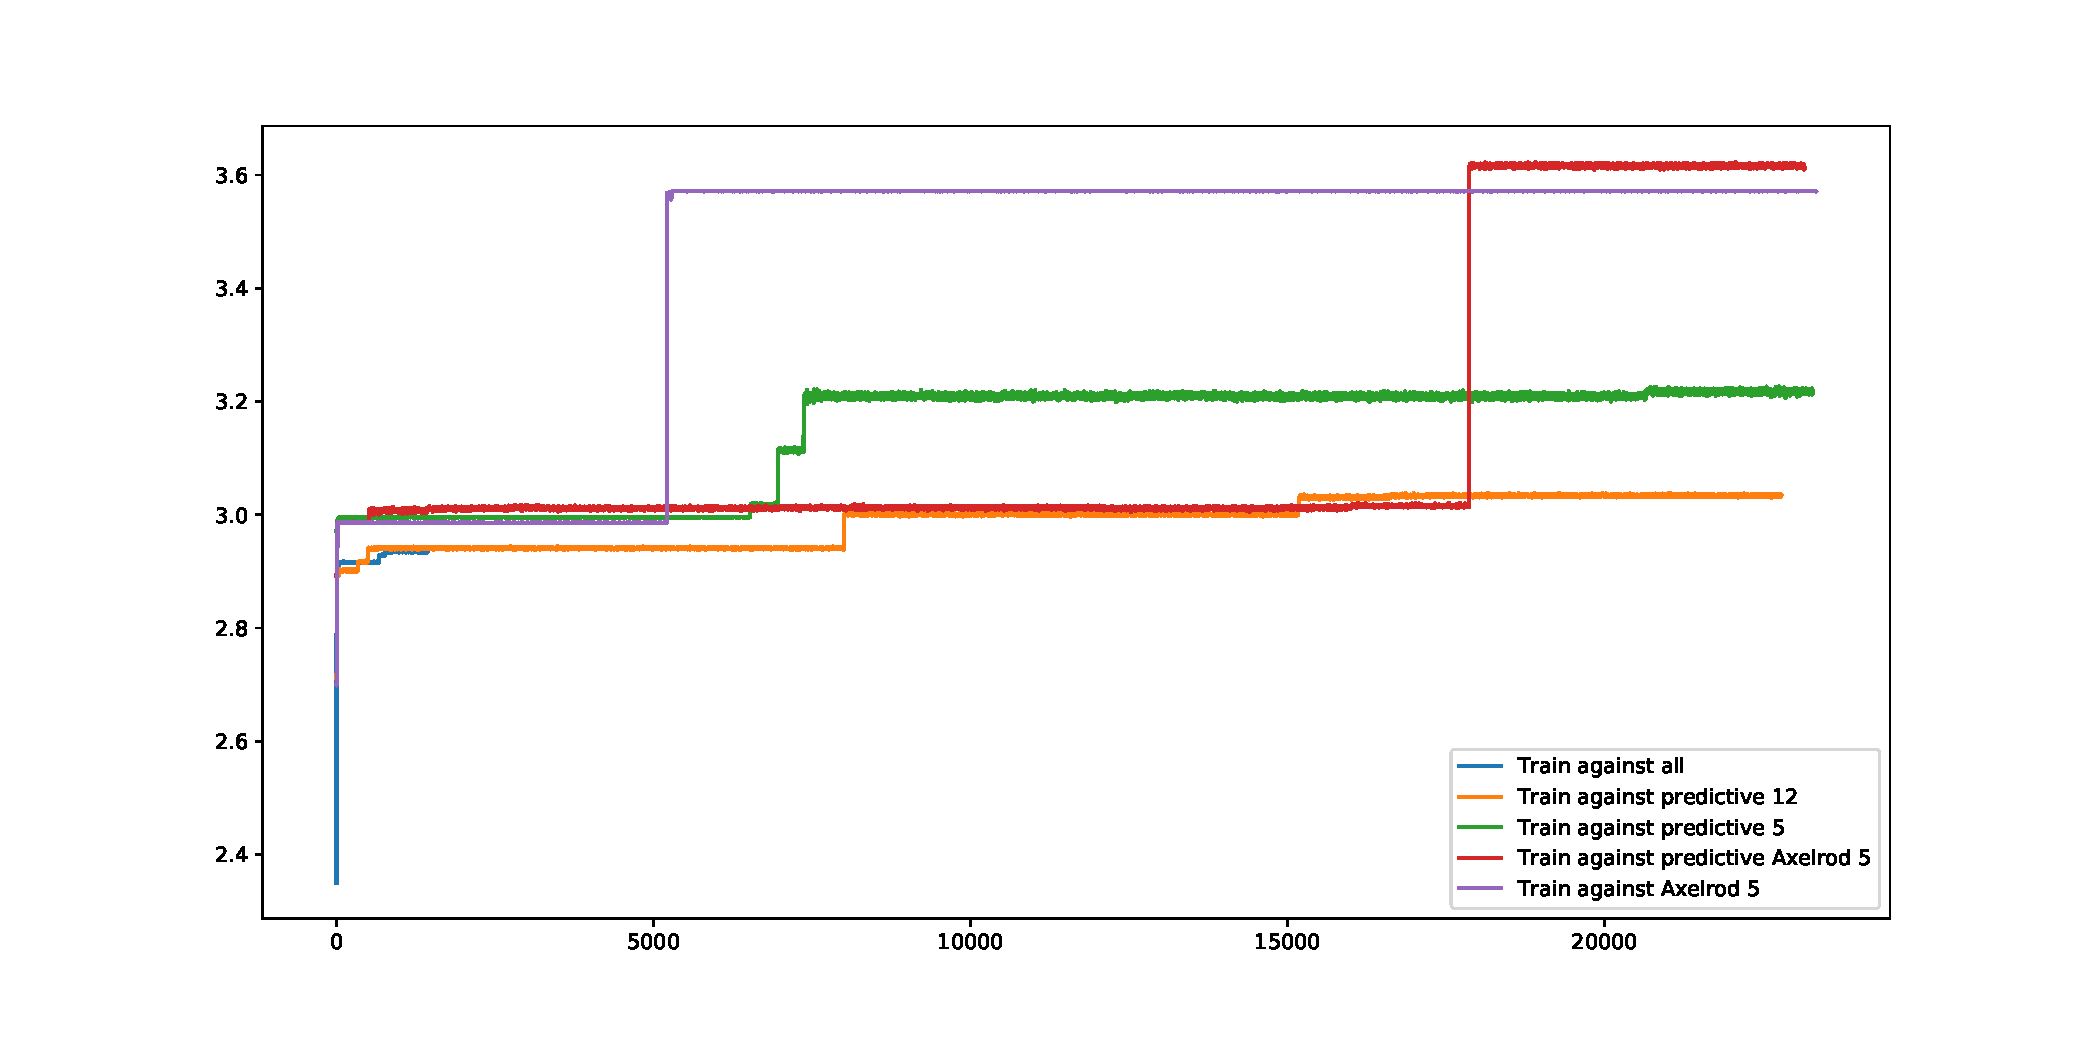
\includegraphics[width=.8\textwidth]{assets/training_data_max_score.pdf}
    \caption{The maximum score per generation over the training periods}
    \label{fig:training_data_max_score}
\end{figure}

The relative score is not necessarily interpretable (the weights of the
particular regression model skew this).
% TODO Add more details

Table~\ref{tbl:original_tournament_with_trained_strategy} shows the results of
the trained strategy in the tournament.

\begin{table}[!hbtp]
        \centering
        \tiny
        \begin{tabular}{lrrrrl}
\toprule
{} &  Cooperation Rate against opponents &  Cooperation Rate from opponents &  Rank &  Score &            Winner \\
Training environment                 &                                     &                                  &       &        &                   \\
\midrule
Full Players                         &                               0.919 &                            0.917 &     1 &  2.933 &  Trained strategy \\
Full Players With Axl                &                               0.946 &                            0.919 &     2 &  2.839 &              k92r \\
Predictive 5 Strategies              &                               0.790 &                            0.746 &    41 &  2.621 &              k92r \\
Representative Strategies            &                               0.599 &                            0.652 &    52 &  2.479 &              k92r \\
Predictive 12 Strategies             &                               0.758 &                            0.656 &    53 &  2.423 &              k92r \\
Predictive With Axelrod 5 Strategies &                               0.777 &                            0.687 &    53 &  2.384 &              k92r \\
\bottomrule
\end{tabular}

        \caption{Results of trained strategy based on environment.}
         \label{tbl:original_tournament_with_trained_strategy}
\end{table}


\subsection{Further tournaments}

% TODO As a brief conclusion show results for these two larger tournaments.

\subsubsection{Running with extortion}\label{sec:run_with_stewart_plotkin}

Since the work of~\cite{Press2012} a lot of interest has been shown to Zero
Determinant strategies. In~\cite{Stewart2012} a small tournament is presented
pitting these against each other. Table~\ref{tbl:sp_tournament_rankings}
shows the rankings of the top 15 strategies when including all the Zero
Determinant strategies from~\cite{Stewart2012} over
25000repetitions.

\begin{table}[!hbtp]
        \centering
        \begin{tabular}{llrrrl}
\toprule
{} &                        Original Author &  Scores &  Rank &  Original Rank & Reproduced Rank \\
\midrule
ZD-GTFT-2 &                                     NA &  2.8366 &     1 &             NA &              NA \\
GTFT      &                                     NA &  2.8214 &     2 &             NA &              NA \\
k92r      &                        Anatol Rapoport &  2.8146 &     3 &              1 &               1 \\
k42r      &                          Otto Borufsen &  2.8046 &     4 &              3 &               2 \\
k75r      &                      Paul D Harrington &  2.7935 &     5 &              8 &               5 \\
k49r      &                               Rob Cave &  2.7894 &     6 &              4 &               4 \\
k44r      &                          William Adams &  2.7840 &     7 &              5 &               3 \\
k68r      &                       Fransois Leyvraz &  2.7717 &     8 &             12 &              10 \\
k41r      &                            Herb Weiner &  2.7648 &     9 &              7 &               8 \\
k32r      &                       Charles Kluepfel &  2.7617 &    10 &             10 &               6 \\
k46r      &                     Graham J Eatherley &  2.7614 &    11 &             14 &              13 \\
k72r      &                      Edward C White Jr &  2.7589 &    12 &             13 &              12 \\
k35r      &                        Abraham Getzler &  2.7506 &    13 &             11 &              11 \\
k84r      &  T Nicolaus Tideman and Paula Chieruzz &  2.7492 &    14 &              9 &               7 \\
k60r      &           Jim Graaskamp and Ken Katzen &  2.7382 &    15 &              6 &               9 \\
\bottomrule
\end{tabular}

        \caption{Top 15 strategies in the tournament composed of the original
                 strategies and the Zero Determinant strategies
                 from~\cite{Stewart2012}}
        \label{tbl:sp_tournament_rankings}
\end{table}

The overall cooperation rate of this tournament is
0.732and the various
cooperation rates are shown in
Figure~\ref{fig:sp_tournament_cooperation_rate_versus_rank} shows the
cooperation rates of each strategy (ordered by rank).

\begin{figure}[!hbtp]
    \centering
    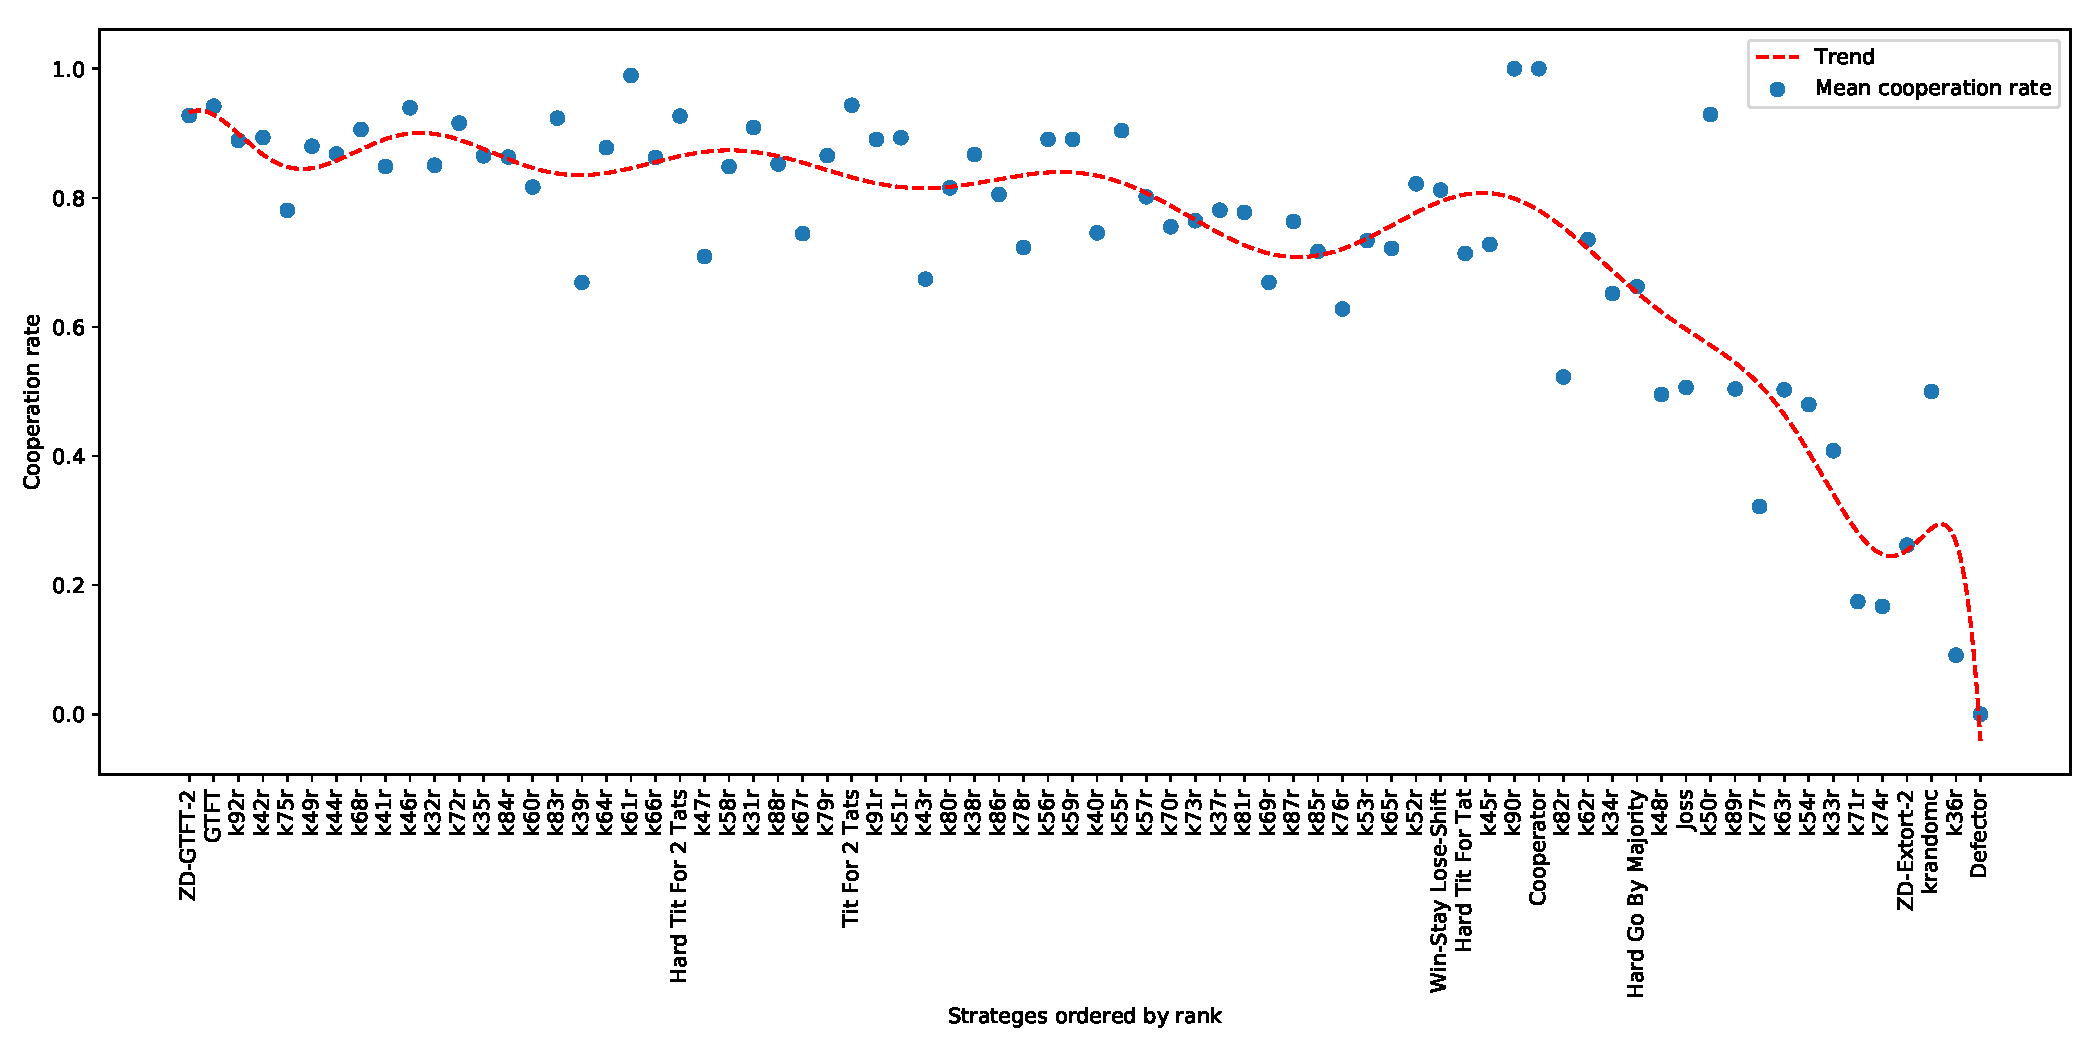
\includegraphics[width=.8\textwidth]{assets/sp_tournament_cooperation_rate_versus_rank.pdf}
    \caption{Cooperation rate versus rank for the Stewart and Poltkin tournament}
    \label{fig:sp_tournament_cooperation_rate_versus_rank}
\end{figure}


\begin{figure}[!hbtp]
    \centering
    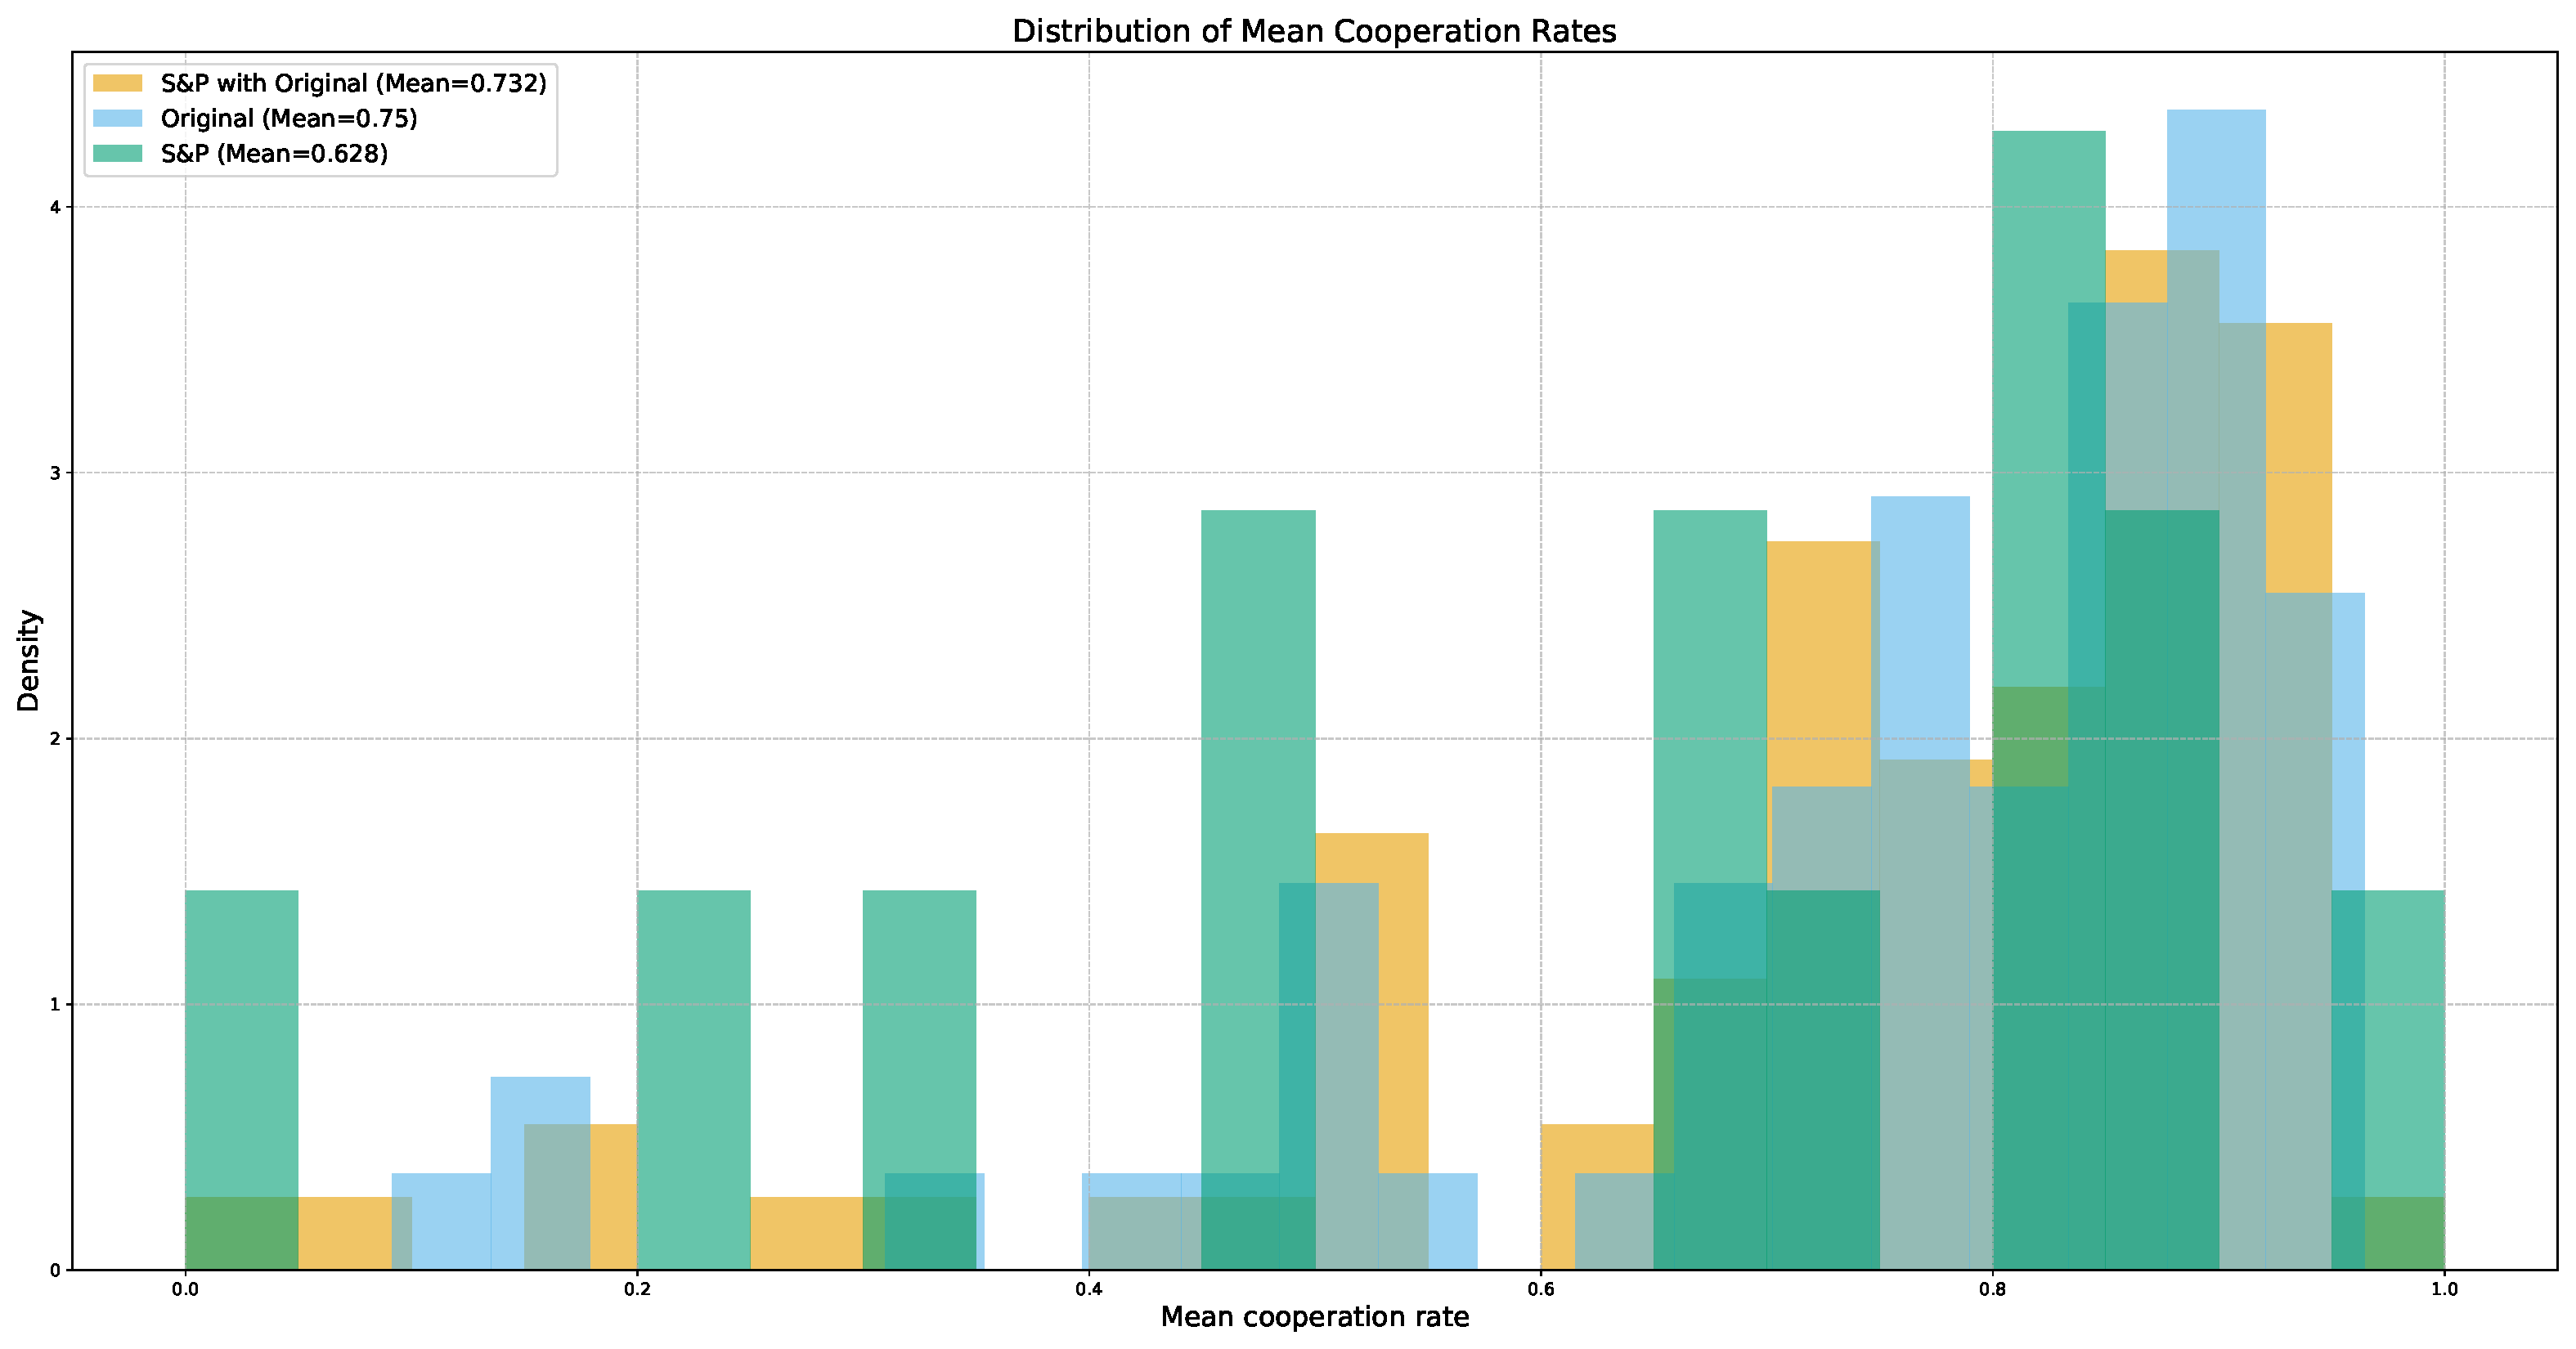
\includegraphics[width=.8\textwidth]{assets/sp_tournament_cooperation_rates.pdf}
    \caption{Distribution of cooperation rates for the Stewart and Plotkin
    tournament}
    \label{fig:sp_tournament_cooperation_rates}
\end{figure}

Figure~\ref{fig:sp_tournament_pairwise_cooperation_rates} shows the pair wise
cooperation rates.

\begin{figure}[!hbtp]
    \centering
    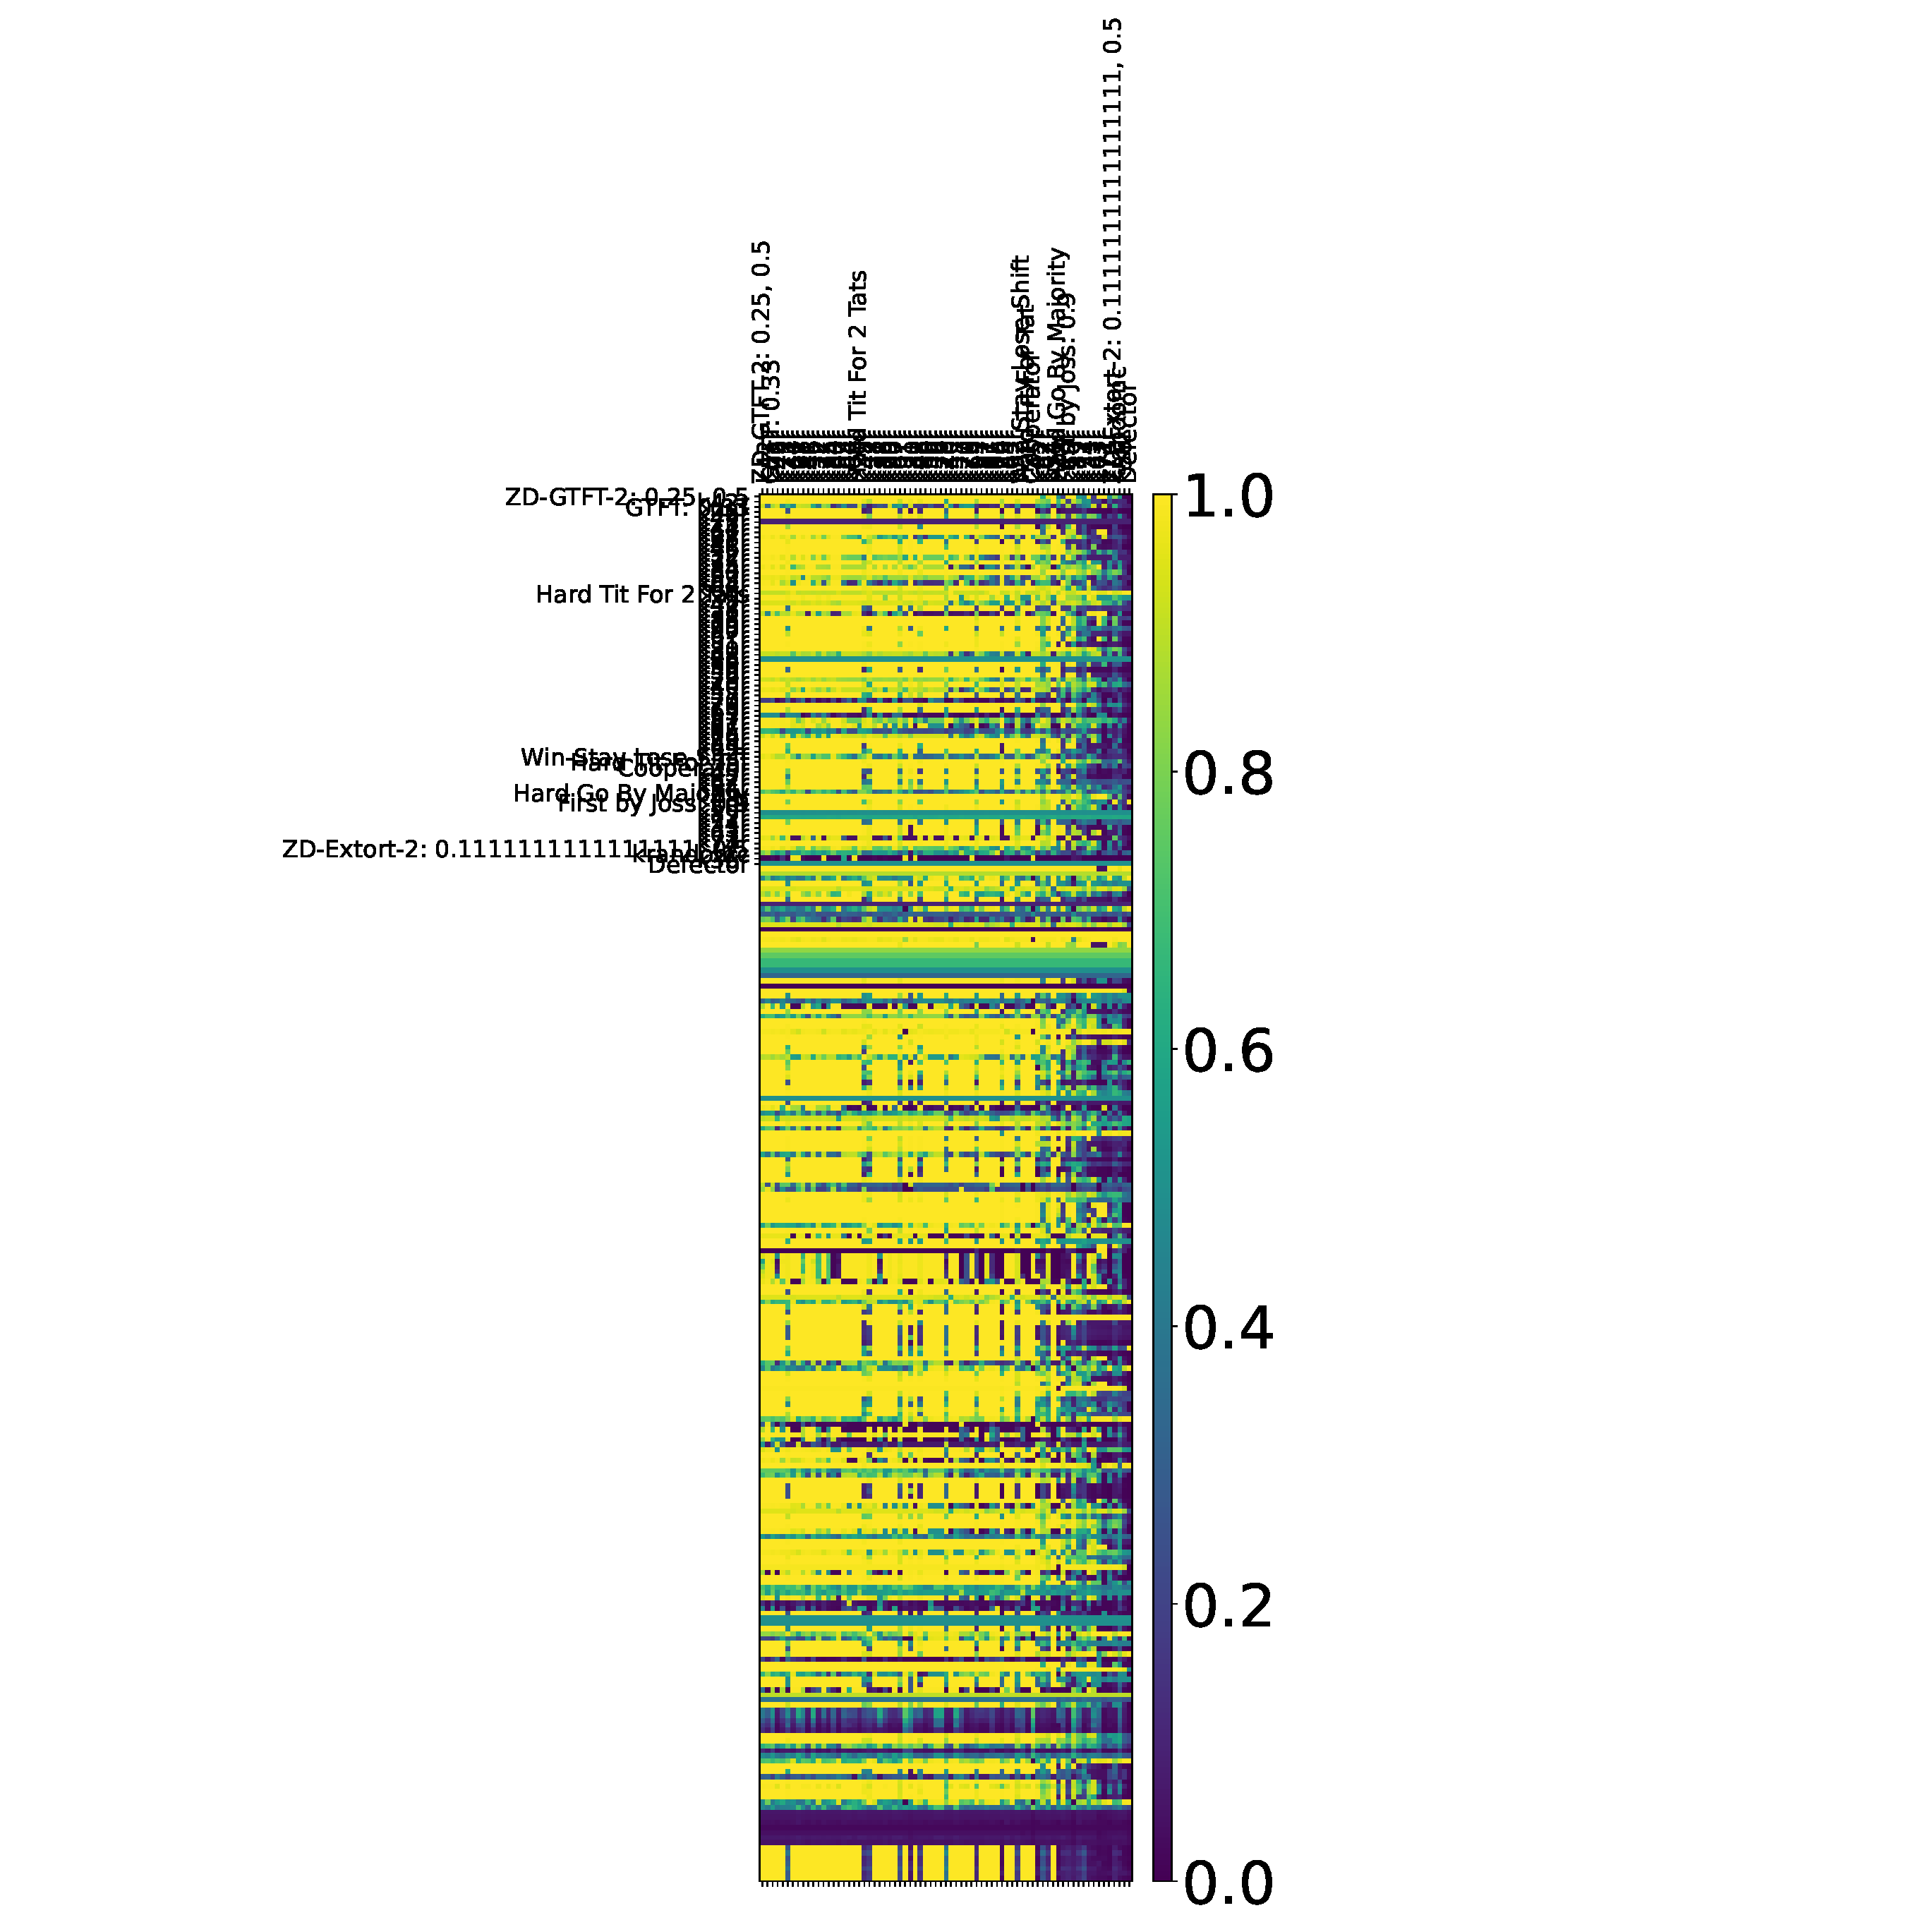
\includegraphics[width=.8\textwidth]{assets/sp_tournament_pairwise_cooperation_rates}
    \caption{Cooperation rates between each pair of players (ordered by rank)
    for the Stewart and Plotkin tournament}
    \label{fig:sp_tournament_pairwise_cooperation_rates}
\end{figure}

\subsubsection{Running a large tournament}\label{sec:run_with_everyone}

Table~\ref{tbl:full_tournament_rankings}
shows the rankings of the top 20 strategies when including all strategies over
4750repetitions.
The cooperation rate for the tournament that pits all the library strategies
against each other (without the Fortran ones) is
0.624\unskip.

\begin{table}[!hbtp]
        \centering
        \footnotesize
        \begin{tabular}{lrrrrrrr}
\toprule
 & Mean Score & Rank & Coop. Rate & Original Rank & Original Coop. Rate & Library Rank & Library Coop. Rate \\
\midrule
EvolvedLookerUp2\_2\_2 & 2.802 & 1 & 0.756 & NA & NA & 1 & 0.736 \\
Evolved HMM 5 & 2.788 & 2 & 0.751 & NA & NA & 2 & 0.742 \\
Omega TFT: 3, 8 & 2.786 & 3 & 0.750 & NA & NA & 12 & 0.725 \\
Evolved ANN 5 & 2.784 & 4 & 0.720 & NA & NA & 3 & 0.713 \\
Evolved ANN & 2.782 & 5 & 0.739 & NA & NA & 5 & 0.727 \\
Evolved FSM 16 & 2.780 & 6 & 0.731 & NA & NA & 4 & 0.713 \\
Evolved FSM 16 Noise 05 & 2.776 & 7 & 0.726 & NA & NA & 6 & 0.717 \\
PSO Gambler 2\_2\_2 & 2.760 & 8 & 0.702 & NA & NA & 7 & 0.692 \\
Original Gradual & 2.757 & 9 & 0.808 & NA & NA & NA & NA \\
PSO Gambler 2\_2\_2 Noise 05 & 2.756 & 10 & 0.740 & NA & NA & 14 & 0.723 \\
PSO Gambler Mem1 & 2.756 & 11 & 0.734 & NA & NA & 9 & 0.728 \\
Evolved FSM 4 & 2.752 & 12 & 0.793 & NA & NA & 10 & 0.777 \\
PSO Gambler 1\_1\_1 & 2.752 & 13 & 0.704 & NA & NA & 8 & 0.702 \\
Gradual & 2.746 & 14 & 0.763 & NA & NA & 15 & 0.793 \\
DBS: 0.75, 3, 4, 3, 5 & 2.739 & 15 & 0.750 & NA & NA & 11 & 0.739 \\
k42r & 2.735 & 16 & 0.820 & 3 & 0.916 & NA & NA \\
Winner12 & 2.733 & 17 & 0.688 & NA & NA & 16 & 0.682 \\
Spiteful Tit For Tat & 2.723 & 18 & 0.691 & NA & NA & 19 & 0.664 \\
k60r & 2.723 & 19 & 0.691 & 6 & 0.844 & NA & NA \\
k85r & 2.716 & 20 & 0.627 & 33 & 0.726 & NA & NA \\
EugineNier: (D,) & 2.713 & 21 & 0.673 & NA & NA & 22 & 0.645 \\
k80r & 2.706 & 22 & 0.723 & 36 & 0.809 & NA & NA \\
k32r & 2.704 & 23 & 0.758 & 10 & 0.873 & NA & NA \\
DoubleCrosser: (D, D) & 2.703 & 24 & 0.693 & NA & NA & 13 & 0.677 \\
k58r & 2.703 & 25 & 0.746 & 21 & 0.852 & NA & NA \\
\bottomrule
\end{tabular}

        \caption{Top 20 strategies in the tournament when using all available
        strategies}
        \label{tbl:full_tournament_rankings}
\end{table}

The overall cooperation rate of this tournament is
0.635and the various
cooperation rates are shown in
Figure~\ref{fig:full_tournament_cooperation_rate_versus_rank} shows the
cooperation rates of each strategy (ordered by rank).

\begin{figure}[!hbtp]
    \centering
    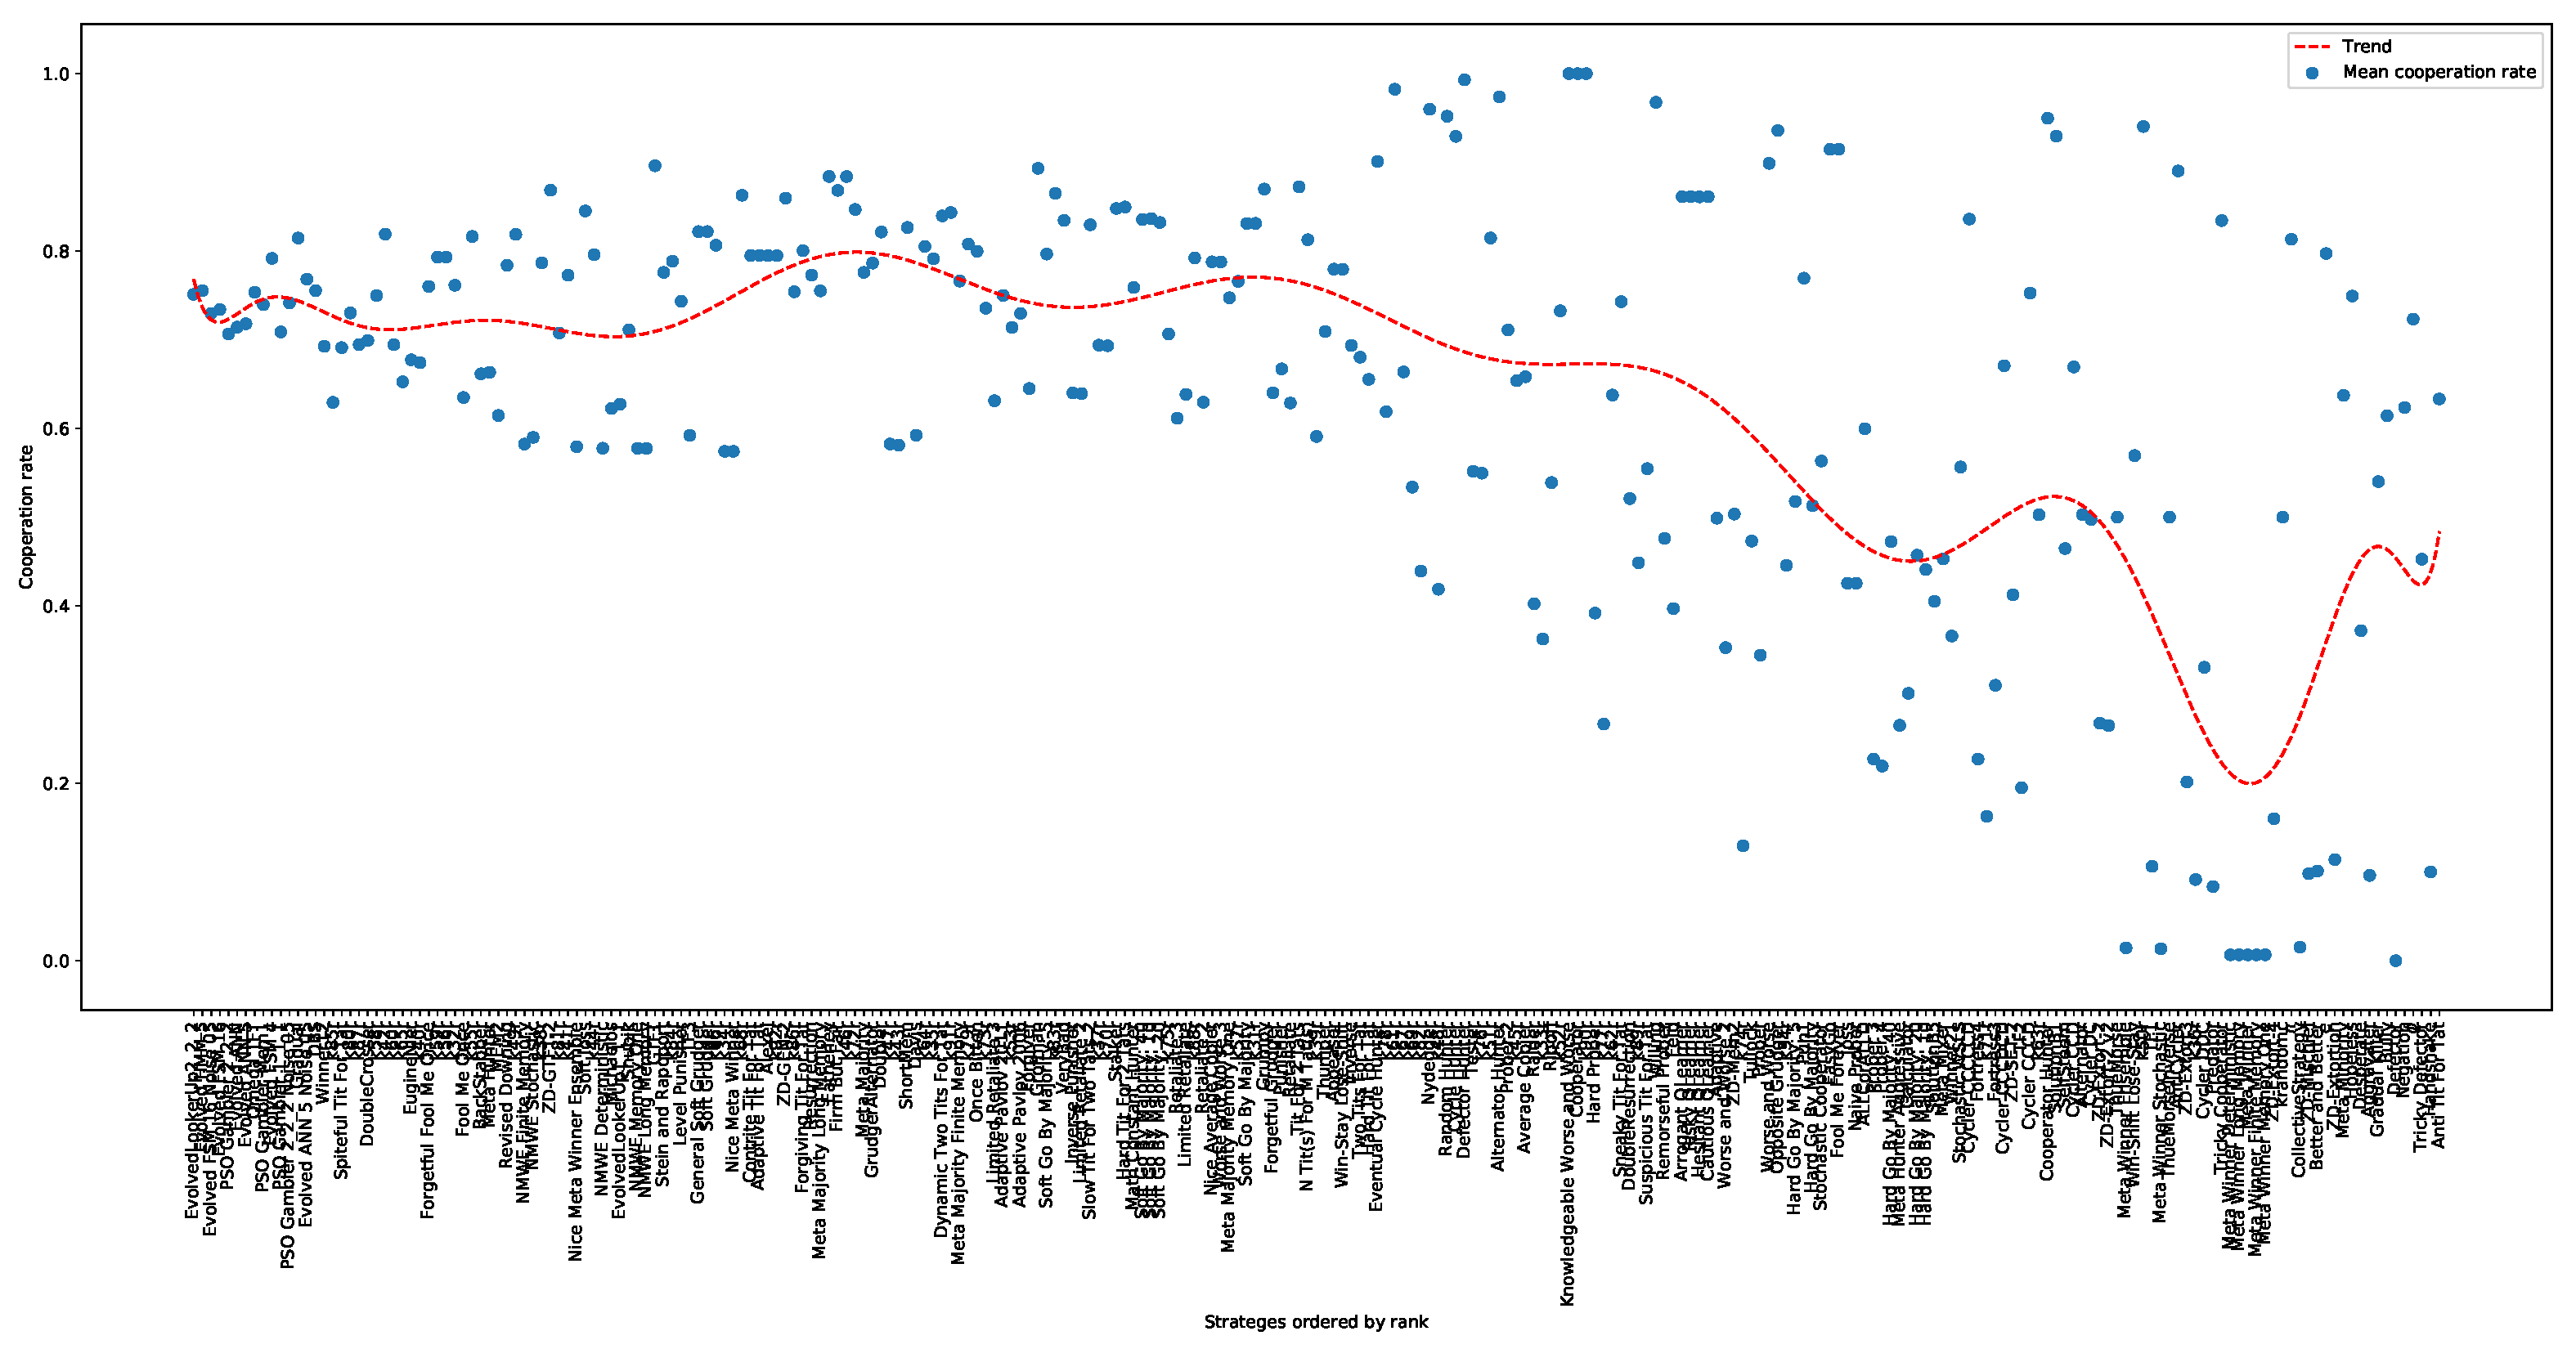
\includegraphics[width=.8\textwidth]{assets/full_tournament_cooperation_rate_versus_rank.pdf}
    \caption{Cooperation rate versus rank for tournament with all available
    strategies}
    \label{fig:full_tournament_cooperation_rate_versus_rank}
\end{figure}

\begin{figure}[!hbtp]
    \centering
    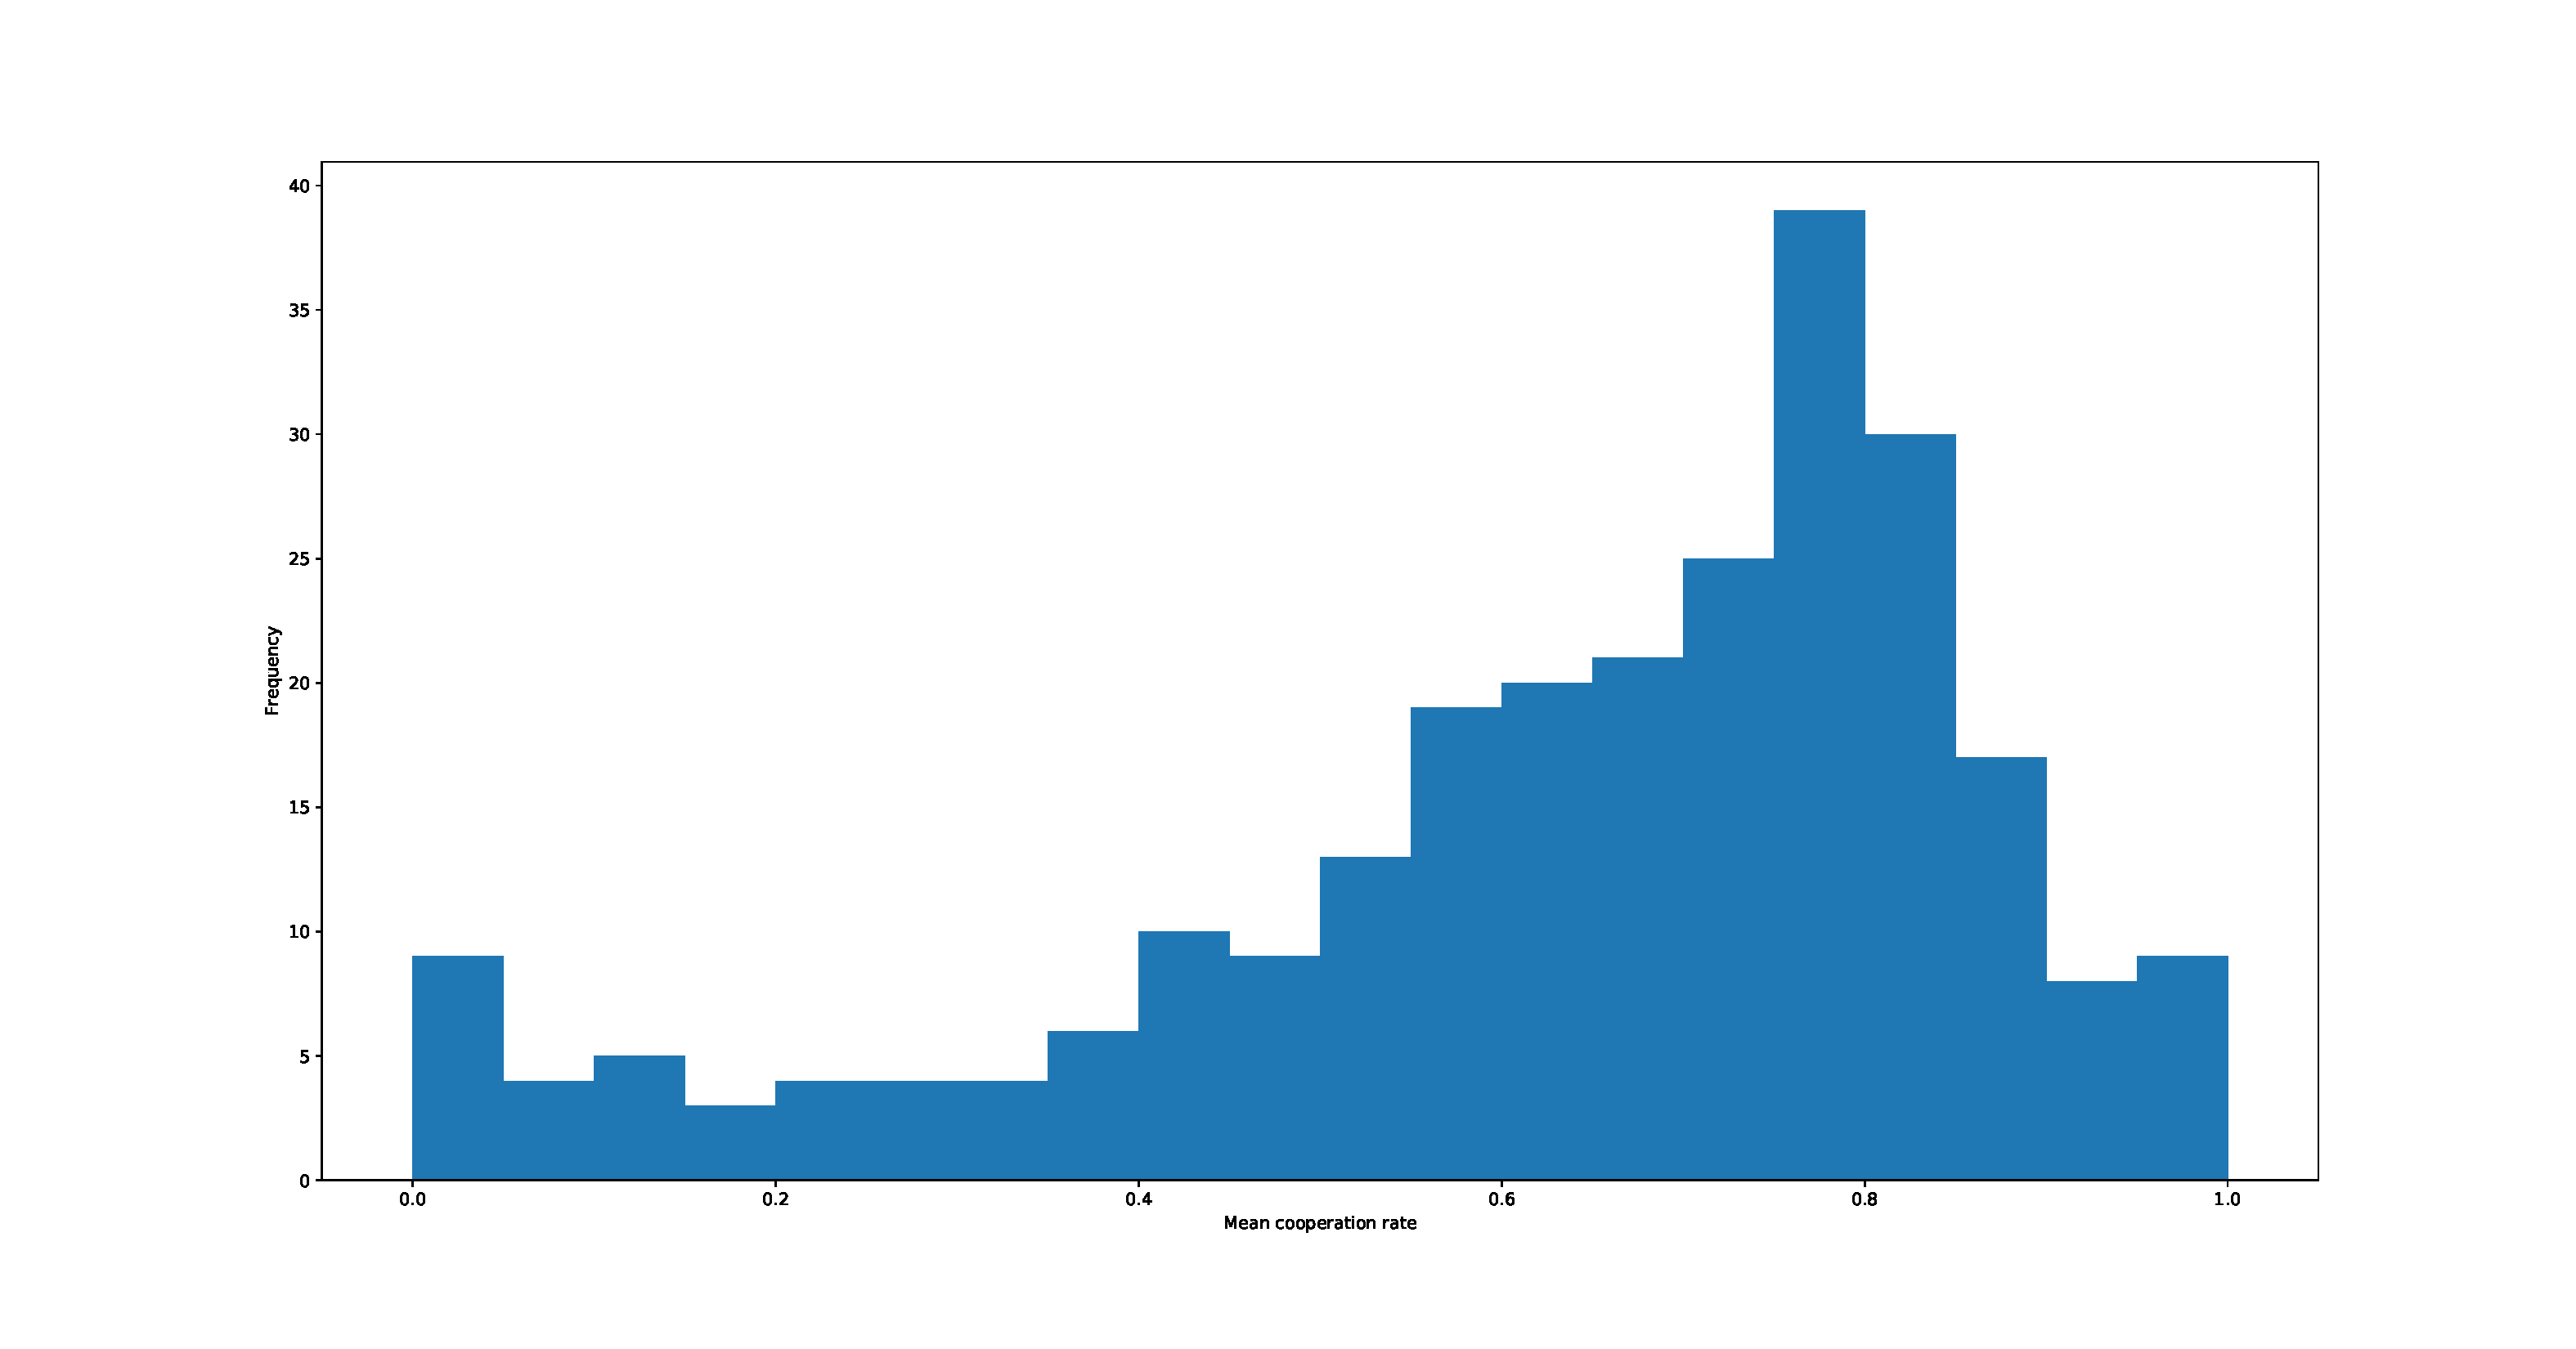
\includegraphics[width=.8\textwidth]{assets/full_tournament_cooperation_rates.pdf}
    \caption{Distribution of cooperation rates for the full tournament.}
    \label{fig:full_tournament_cooperation_rates}
\end{figure}

Figure~\ref{fig:full_tournament_pairwise_cooperation_rates} shows the pair wise
cooperation rates.

\begin{figure}[!hbtp]
    \centering
    \includegraphics[width=.8\textwidth]{assets/full_tournament_pairwise_cooperation_rates}
    \caption{Cooperation rates between each pair of players (ordered by rank)
    for tournament with all available strategies}
    \label{fig:full_tournament_pairwise_cooperation_rates}
\end{figure}

\section{Conclusion}\label{sec:conclusion}

\section*{Acknowledgements}

% TODO Write appendices for the Axelrod strategies

\bibliographystyle{plain}
\bibliography{bibliography.bib}

\appendix

\section{List of original players}\label{app:list_of_original_players}


\begin{multicols}{2}
    \begin{enumerate}
            \item k31r - Original rank: 23. Authored by Gail Grisell
\item k32r - Original rank: 10. Authored by Charles Kluepfel
\item k33r - Original rank: 59. Authored by Harold Rabbie
\item k34r - Original rank: 52. Authored by James W Friedman
\item k35r - Original rank: 11. Authored by Abraham Getzler
\item k36r - Original rank: 63. Authored by Roger Hotz
\item k37r - Original rank: 37. Authored by George Lefevre
\item k38r - Original rank: 34. Authored by Nelson Weiderman
\item k39r - Original rank: 25. Authored by Tom Almy
\item k40r - Original rank: 35. Authored by Robert Adams
\item k41r - Original rank: 7. Authored by Herb Weiner
\item k42r - Original rank: 3. Authored by Otto Borufsen
\item k43r - Original rank: 39. Authored by R D Anderson
\item k44r - Original rank: 5. Authored by William Adams
\item k45r - Original rank: 50. Authored by Michael F McGurrin
\item k46r - Original rank: 14. Authored by Graham J Eatherley
\item k47r - Original rank: 16. Authored by Richard Hufford
\item k48r - Original rank: 53. Authored by George Hufford
\item k49r - Original rank: 4. Authored by Rob Cave
\item k50r - Original rank: 54. Authored by Rik Smoody
\item k51r - Original rank: 18. Authored by John William Colbert
\item k52r - Original rank: 48. Authored by David A Smith
\item k53r - Original rank: 45. Authored by Henry Nussbacher
\item k54r - Original rank: 58. Authored by William H Robertson
\item k55r - Original rank: 42. Authored by Steve Newman
\item k56r - Original rank: 38. Authored by Stanley F Quayle
\item k57r - Original rank: 31. Authored by Rudy Nydegger
\item k58r - Original rank: 21. Authored by Glen Rowsam
\item k59r - Original rank: 40. Authored by Leslie Downing
\item k60r - Original rank: 6. Authored by Jim Graaskamp and Ken Katzen
\item k61r - Original rank: 2. Authored by Danny C Champion
\item k62r - Original rank: 51. Authored by Howard R Hollander
\item k63r - Original rank: 57. Authored by George Duisman
\item k64r - Original rank: 17. Authored by Brian Yamachi
\item k65r - Original rank: 47. Authored by Mark F Batell
\item k66r - Original rank: 20. Authored by Ray Mikkelson
\item k67r - Original rank: 27. Authored by Craig Feathers
\item k68r - Original rank: 12. Authored by Fransois Leyvraz
\item k69r - Original rank: 29. Authored by Johann Joss
\item k70r - Original rank: 32. Authored by Robert Pebly
\item k71r - Original rank: 60. Authored by James E Hall
\item k72r - Original rank: 13. Authored by Edward C White Jr
\item k73r - Original rank: 41. Authored by George Zimmerman
\item k74r - Original rank: 61. Authored by Edward Friedland
\item k75r - Original rank: 8. Authored by Paul D Harrington
\item k76r - Original rank: 46. Authored by David Gladstein
\item k77r - Original rank: 55. Authored by Scott Feld
\item k78r - Original rank: 19. Authored by Fred Mauk
\item k79r - Original rank: 26. Authored by Dennis Ambuehl and Kevin Hickey
\item k80r - Original rank: 36. Authored by Robyn M Dawes and Mark Batell
\item k81r - Original rank: 43. Authored by Martyn Jones
\item k82r - Original rank: 49. Authored by Robert A Leyland
\item k83r - Original rank: 15. Authored by Paul E Black
\item k84r - Original rank: 9. Authored by T Nicolaus Tideman and Paula Chieruzz
\item k85r - Original rank: 33. Authored by Robert B Falk and James M Langsted
\item k86r - Original rank: 28. Authored by Bernard Grofman
\item k87r - Original rank: 44. Authored by E E H Schurmann
\item k88r - Original rank: 22. Authored by Scott Appold
\item k89r - Original rank: 56. Authored by Gene Snodgrass
\item k90r - Original rank: 24. Authored by John Maynard Smith
\item k91r - Original rank: 30. Authored by Jonathan Pinkley
\item k92r - Original rank: 1. Authored by Anatol Rapoport
\item krandomc - Original rank: 62. Authored by None

    \end{enumerate}
\end{multicols}


\end{document}
